\section{Parameterization}\label{model.par}
As described in \sref{intro.model.param}, model parameterization involves
specification of model parameter values, such as proportions, probabilities, rates, and ratios,
including stratified values to reflect heterogeneity,
and sampling distributions to reflect uncertainty.
Proportions and probabilities were generally modelled using
a beta approximation of the binomial distribution (BAB, see \sref{app.math.distr.bab}),
while rates and ratios were generally modelled using
a gamma, skewnormal, or inverse gaussian distribution.
%---------------------------------------------------------------------------------------------------
\paragraph{Notation}
If $X$ is a parameter stratified by dimensions $a,b,c$,
then $X_{ab_{1}c_{23}}$ denotes the values of $X$ for
a particular but \emph{unspecified} stratum of $a$,
the \emph{specific} stratum $b = 1$,
and the \emph{aggregated} strata $c = 2,3$
(the aggregating operation is context-dependent, \eg sum for probabilities).
Additionally, the indices $sihc$ from Table~\ref{tab:model.dims} denote ``self'' strata,
whereas $s'i'h'c'$ denote ``other'' strata --- \ie individuals' partners.%
\footnote{\label{foot:code.note}%
  In the code: R uses one-based indexing, which match the notation here directly,
  while Python uses zero-based indexing, which therefore appear as $i \rightarrow i-1$ in the code.
  Also, the model code reorders states in the ART Cascade dimension for computational efficiency,
  with $c={}$1:~Undiagnosed; 2:~Diagnosed; 3:~Virally~Un-suppressed; 4:~On~ART; 5:~Virally~Suppressed.}
Finally, I re-use several dummy variables throughout the chapter:
$\rho$ for proportions, $\lambda$ for rates, $T$ for time periods, and $f$ for constants.
%===================================================================================================
\subsection{Risk Heterogeneity Among FSW}\label{model.par.fsw}
HIV transmission models which include FSW rarely sub-stratify this population, such as to reflect
differential HIV risk or distinct typologies of sex work \cite{Blanchard2008,Scorgie2012};
yet such heterogeneities likely influence transmission dynamics.
Among the studies identified in Chapter~\ref{sr},
only three sub-stratified FSW by risk-related factors:
\citet{Cremin2017} defined three levels of risk via regression analysis,
\citet{Low2015} distinguished between occasional and full-time FSW, while
\citet{Shannon2015} sub-stratified FSW by
work environment, violence exposure, and context-specific structural factors.
Seven other studies, reflecting two unique models \cite{Johnson2012,Maheu-Giroux2017},
employed age stratification of all activity groups, including FSW;
these models had several risk-related parameters which varied by age.
\par
The model structure here (Figure~\ref{fig:model.risk})
was designed to capture \emph{within}-FSW risk heterogeneity.
The objective of the following analysis was therefore to parameterize
lower versus higher risk FSW.
I sought to define these groups based on biobehavioural and/or contextual factors
which are demonstrably associated with HIV risk,
and which can be mechanistically incorporated into a transmission model ---
\ie through the force of infection equation.
Later, the parameterization of these groups was validated through model fitting
to relative differences in HIV prevalence \sref{model.cal.targ.prev}.
\par
Many cross-sectional studies of HIV among FSW quantify
the association of risk factors with HIV serostatus
\cite{Aklilu2001,Dunkle2005,Scorgie2012,Jonas2020}.
However, serostatus reflects cumulative risk exposure,
whereas sexual risk behaviour is dynamic \cite{Watts2010,vanWees2020},
as is use of prevention resources \cite{Roberts2020}.
For example, while HIV prevalence often increases with age,
HIV incidence among women can peak shortly after sexual debut \cite{Dellar2015}.
Thus, risk factors associated with HIV serostatus are not necessarily
mechanistically related to HIV acquisition.
Indeed, FSW may reduce risk behaviours in response to seroconversion \cite{McClelland2006}.
Cohort studies that measure incidence
can help identify risk factors for HIV acquisition \cite{McKinnon2015,Nouaman2022},
but large sample sizes are often required to accurately estimate overall incidence rate,
let alone risk factors \cite{Priddy2011}.
%---------------------------------------------------------------------------------------------------
\subsubsection{FSW Survey Data}\label{model.par.fsw.data}
Three surveys, in
2011 \cite{Baral2014} (N = 325),
2014 \cite{EswKP2014} (N = 781), and
2021 \cite{EswIBBS2022} (N = 676)
provide HIV and biobehavioural data on FSW in Eswatini.
The 2011 survey employed respondent driven sampling (RDS, details in \cite{Yam2013}),
as did the 2021 survey.
The 2014 survey employed venue-based snowball sampling, based on the
Priorities for Local AIDS Control Efforts (PLACE) methodology,
which aims to identify areas of higher incidence \cite{Weir2005}.
I analyzed the individual-level data from 2011 and 2014 (data from 2021 not yet available)
to explore the potential association of biobehavioural factors with HIV risk,
so that such factors could then be used to distinguish between
lower risk versus higher risk FSW.
%---------------------------------------------------------------------------------------------------
\subsubsection{HIV Status}\label{model.par.fsw.hiv}
Only the 2011 and 2021 studies included serologic testing for HIV.
Among those tested in 2011 (N = 317, 98\%), 70\% were \hivp,
yielding RDS-adjusted prevalence estimate of 61\% (CI: 51--71\%) \cite{Baral2014}.
Among serologically \hivn, 11\% self-reported \hivp status (false positive), and
among serologically \hivp, 26\% self-reported \hivn status (false negative or undiagnosed).
Overall, self-reported HIV status underestimated HIV prevalence in 2011
by a factor of approximately 0.78 (55~vs~70\%).
Unadjusted HIV prevalence in 2021 was 58.8\%,
with 88\% (363/411) reporting previous awareness of \hivp status.
\par
In 2014, self-reported HIV prevalence was 38\% among respondents who reported (85\%).
This 38\% is surprisingly low considering that
the PLACE methodology explicitly aimed to sample venues
with higher HIV incidence \cite{Weir2005}, and 2014 versus 2011 respondents
were older (median 27 \vs 25 years), % 2021 median: 28
had been selling sex longer (median 5 \vs 4 years), % 2021: 6
and tested more frequently (87 \vs 75\% tested at least once in the past year, % 2021: 75
82 \vs 63\% among self-reported \hivn).
Perhaps the differences are attributable to the sampling methodology.
Among respondents who self-reported \hivp status,
the 2014 survey also asked for age of HIV diagnosis (6\% missing).
Age of HIV diagnosis supports crude time-to-event analysis (next section),
which can account for confounding by age and censoring,
as compared to logistic regression on HIV status,
keeping in mind the limitations of self-reported HIV status.
%---------------------------------------------------------------------------------------------------
\subsubsection{Risk Factors}\label{model.par.fsw.fac}
Next, I explored the potential association of risk factors with HIV
via the following three models:%
\footnote{Logistic regression models were implemented using \texttt{lrm} from:
  \hreftt{cran.r-project.org/package=rms}.\\
Cox proportional hazards models were implemented using \texttt{coxaalen} from:
  \hreftt{cran.r-project.org/package=coxinterval}.}
\begin{enumerate}
  \item Logistic regression on serologic HIV status (2011 data)
  \item Logistic regression on self-reported HIV status (2014 data)
  \item Cox proportional hazards for interval-censored time to HIV infection,
    with interval from self-reported sex work debut 
    to either self-reported time of HIV diagnosis or survey date (2014 data);
    Figure~\ref{fig:fsw.tte.interval} illustrates
    the four potential censoring cases in this framework.
\end{enumerate}
An important limitation to all models is that
risk factors reported by FSW at the time of survey
are assumed to be fixed characteristics of the respondents,
rather than dynamic characteristics that vary over time.
Additionally, respondents with any missing variables for each individual model
were excluded from that model. % TODO: (%)
\begin{figure}
  \centering
  \includegraphics[scale=1]{tte.interval}
  \caption{Illustration of time-to-event analysis framework
    for cross-sectional FSW survey data}
  \label{fig:fsw.tte.interval}
  \floatfoot{
    $\bm{\times}$: HIV infection;
    SW: time of sex work debut;
    Dx: time of HIV diagnosis.}
\end{figure}
\par
Risk factors were selected based on
prior knowledge of plausible mechanistic influence on HIV incidence and/or prevalence.
The risk factors explored are summarized in Table~\ref{tab:fsw.stats},
including univariate and multivariate association under each model.
Variable selection for multivariate models
was performed using backward selection as described by \citet{Lawless1978},
using a $p \le 0.1$ (per variable) threshold for stepwise variable retention.
Estimated conditional effects of
variables retained in the multivariate logistic regression models
are illustrated in Figure~\ref{fig:fsw.lr}.
\begin{table}
  \centering
  \caption{Risk factors explored for association with \hivp status among FSW in Eswatini}
  \label{tab:fsw.stats}
  \centerline{%
\small%
\begin{tabular}{lcccccccccccc}
  \toprule
  & \multicolumn{4}{c}{2011 LR}
  & \multicolumn{4}{c}{2014 LR}
  & \multicolumn{4}{c}{2014 CPH} \\
  \cmidrule(rl){2-5}\cmidrule(rl){6-9}\cmidrule(rl){10-13}
  & \multicolumn{2}{c}{Univar} & \multicolumn{2}{c}{Multivar}
  & \multicolumn{2}{c}{Univar} & \multicolumn{2}{c}{Multivar}
  & \multicolumn{2}{c}{Univar} & \multicolumn{2}{c}{Multivar} \\
  \cmidrule(rl){2-3}\cmidrule(rl){4-5}\cmidrule(rl){6-7}\cmidrule(rl){8-9}\cmidrule(rl){10-11}\cmidrule(rl){12-13}
  Factor                          &  OR  &   p   &  OR  &   p    &  OR  &   p    &  OR  &   p    &  HR  &   p    &  HR  &   p    \\
  \midrule                        % 2011 LR uni  % 2011 LR multi % 2014 LR uni   % 2014 LR multi % 2014 CPH uni  % 2014 CPH multi
  Age\tn{a}                       & 1.11 & \vsig & ---  &  ---   & 1.14 & \vsig  & 1.15 & \vsig  & 1.09 & \vsig  & 1.09 & \vsig  \\
  Years selling sex\tn{a}         & 1.13 & \vsig & 1.13 & \vsig  & 1.12 & \vsig  & ---  &  ---   & 1.08 & \vsig  & ---  &  ---   \\
  Monthly sex work income\tn{b}   & 0.98 & 0.155 & ---  &  ---   & 0.98 & 0.097  & 0.97 & 0.084  & 0.98 & 0.019\s& 0.97 & 0.001\s\\[1ex]
  Non-paying partners\tn{c}       & 0.88 & 0.307 & ---  &  ---   & 1.07 & 0.233  & ---  &  ---   & 1.05 & 0.312  & ---  &  ---   \\
  Monthly new clients\tn{c}       & 1.01 & 0.412 & ---  &  ---   & 1.05 & \vsig  & 1.07 & \vsig  & 1.04 & \vsig  & 1.04 & \vsig  \\
  Monthly regular clients\tn{c}   & 1.01 & 0.351 & ---  &  ---   & 1.03 & 0.002  & ---  &  ---   & 1.02 & \vsig  & 1.02 & 0.034\s\\[1ex]
  Non-paying condom use\tn{d}     & 0.90 & 0.703 & ---  &  ---   & 0.90 & 0.673  & ---  &  ---   & 0.92 & 0.677  & ---  &  ---   \\
  New client condom use\tn{d}     & 0.60 & 0.100 & ---  &  ---   & 0.48 & 0.006\s& 1.25 & 0.599  & 0.56 & 0.004\s& ---  &  ---   \\
  Regular client condom use\tn{d} & 0.58 & 0.110 & ---  &  ---   & 0.39 & \vsig  & 0.35 & 0.004\s& 0.49 & \vsig  & 0.50 & \vsig  \\[1ex]
  Any anal sex past month         & 0.97 & 0.896 & ---  &  ---   & 1.89 & 0.015\s& ---  &  ---   & 1.57 & 0.015\s& 1.27 & 0.260  \\
  Any STI symptoms past year      & 2.29 & \vsig & 2.41 & \vsig  & 2.75 & \vsig  & 2.80 & \vsig  & 2.17 & \vsig  & 2.05 & \vsig  \\
  \bottomrule
\end{tabular}}
% TODO: HIV status?
\floatfoot{\raggedright
  \tnt[a]{OR per year};
  \tnt[b]{OR per Swati lilangeni per month};
  \tnt[c]{OR per partner};
  \tnt[d]{2011: always vs not always, 2014: at last sex}.
  --- indicates variable was not selected in the multivariate model.
  LR: logistic regression on HIV$+/-$ status;
  CPH: Cox proportional hazards on time to self-reported HIV seroconversion.
  OR: odds ratio; HR: hazard ratio; p: p-value.
  2011 data based on serologic HIV test;
  2014 data based on self-reported HIV status, age of sex work debut, and age of HIV diagnosis.
}
\end{table}
\begin{figure}
  \begin{subfigure}{0.4\linewidth}
    \centering
    \includegraphics[width=\linewidth]{fsw-survey-2011-lr.pdf}
    \caption{2011 (serologic HIV status)}
  \end{subfigure}%
  \begin{subfigure}{0.6\linewidth}
    \centering
    \includegraphics[width=\linewidth]{fsw-survey-2014-lr.pdf}
    \caption{2014 (self-reported HIV status)}
  \end{subfigure}
  \caption{Predicted conditional effects (probability)
    of significant variables in multivariate logistic regression models
    from 2011 and 2014 surveys}
  \label{fig:fsw.lr}
  \floatfoot{\raggedright
    sti.symp: any STI symptoms past year;
    y.ss: years selling sex;
    cli.new.mo: monthly new clients;
    sw.income.mo: monthly sex work income.
    Conditional probabilities shown for fixed covariates at arbitrary values.}
\end{figure}
\par
Following variable selection, each multivariate model was used to predict
the total \hivp status odds ratio (logistic) or HIV incidence hazard ratio (Cox)
for each respondent in the respective survey ---
\ie $e^{X_i\,\beta}$ for respondent $i$ ---
representing an overall ``risk score'' under each model.
Respondents were then stratified into the top 20\% and bottom 80\% by these risk scores.
The values of each variable were compared between these two strata
using a test for the ratio of the means \cite{Tamhane2004}
to support model parameterization;
these ratios are summarized in Table~\ref{tab:fsw.ratios},
and the distributions of variable values are illustrated in
Figures~\ref{fig:fsw.f.2011}~and~\ref{fig:fsw.f.2014}.
\begin{table}
  \centering
  \caption{Ratios of HIV risk factor variables among higher \vs lower risk FSW in Eswatini}
  \label{tab:fsw.ratios}
  \centerline{\footnotesize%
\begin{tabular}{lcccccc}
  \toprule
  & \multicolumn{2}{c}{2011 LR}
  & \multicolumn{2}{c}{2014 LR}
  & \multicolumn{2}{c}{2014 CPH} \\
  \cmidrule(rl){2-3}\cmidrule(rl){4-5}\cmidrule(rl){6-7}
  Factor                            &  High / Low   &   Ratio (95\% CI)   &  High / Low   &   Ratio (95\% CI)   &   High / Low   &   Ratio (95\% CI)   \\
  \midrule
  Age                               & 31.8  / 24.7  & 1.29 (1.22, 1.36)\s & 32.6  / 26.2  & 1.24 (1.20, 1.28)\s &  33.5  / 26.6  & 1.26 (1.21, 1.31)\s \\
  Years selling sex                 & 11.3  /  4.03 & 2.81 (2.41, 3.25)\s & 10.0  /  5.47 & 1.83 (1.64, 2.03)\s &  10.2  /  5.83 & 1.75 (1.54, 1.98)\s \\
  Monthly sex work income\tn{a}     & 15.1  / 15.2  & 1.00 (0.86, 1.15)   &  6.77 /  7.06 & 0.96 (0.82, 1.11)   &   6.32 /  7.28 & 0.87 (0.73, 1.02)   \\[1ex]
  Non-paying partners               &  1.42 /  1.43 & 0.99 (0.81, 1.19)   &  1.56 /  1.11 & 1.40 (1.11, 1.72)\s &   1.53 /  1.19 & 1.29 (0.98, 1.62)   \\
  Monthly new clients               &  5.50 /  6.98 & 0.79 (0.49, 1.15)   &  8.39 /  4.15 & 2.02 (1.63, 2.44)\s &   8.36 /  4.41 & 1.90 (1.43, 2.39)\s \\
  Monthly regular clients           &  9.35 /  9.05 & 1.03 (0.69, 1.42)   & 11.1  /  8.25 & 1.35 (1.13, 1.57)\s &  12.4  /  8.61 & 1.44 (1.18, 1.71)\s \\[1ex]
  Non-paying condom use\tn{bc}      &  0.26 /  0.35 & 0.73 (0.40, 1.11)   &  0.77 /  0.81 & 0.95 (0.84, 1.06)   &   0.76 /  0.81 & 0.95 (0.81, 1.08)   \\
  New client condom use\tn{bc}      &  0.68 /  0.76 & 0.89 (0.73, 1.06)   &  0.79 /  0.91 & 0.86 (0.79, 0.94)\s &   0.74 /  0.94 & 0.79 (0.69, 0.88)\s \\
  Regular client condom use\tn{bc}  &  0.38 /  0.46 & 0.83 (0.45, 1.28)   &  0.67 /  0.91 & 0.74 (0.65, 0.82)\s &   0.60 /  0.92 & 0.65 (0.55, 0.75)\s \\[1ex]
  Any anal sex past month           &  0.59 /  0.41 & 1.41 (1.06, 1.84)\s &  0.17 /  0.07 & 2.43 (1.47, 3.85)\s &   0.23 /  0.07 & 3.24 (1.95, 5.34)\s \\
  Any STI symptoms past year\tn{c}  &  0.79 /  0.43 & 1.86 (1.54, 2.25)\s &  0.59 /  0.15 & 3.94 (3.15, 5.03)\s &   0.61 /  0.17 & 3.67 (2.87, 4.79)\s \\[1ex]
  HIV prevalence\tn{d}              &  0.94 /  0.64 & 1.46 (1.30, 1.63)\s &  0.66 /  0.29 & 2.29 (1.92, 2.75)\s &   0.71 /  0.31 & 2.32 (1.94, 2.80)\s \\
  \bottomrule
\end{tabular}}
\floatfoot{\raggedright
  High / Low: mean variable value among higher / lower risk groups, as defined by
  the top 20\% / bottom 80\% in multivariable model-predicted risk score:
  odds ratio from logistic regression (LR);
  hazards ratio from Cox proportional hazards (CPH).
  \tnt[a]{Swati lilangeni per month};
  \tnt[b]{2011: always \vs not always, 2014: did use condom at last sex};
  \tnt[c]{proportion of respondents};
  \tnt[d]{2011: serologic HIV status; 2014: self-reported HIV status};
  \tnt[*]{statistically significant, $p < 0.05$}.
}
\end{table}
%---------------------------------------------------------------------------------------------------
\subsubsection{Discussion}\label{model.par.fsw.disc}
TODO
% - novelty of 20/80 split by risk -> parameterization
% - compare to other risk scores of SSA women: Balkus2016; Willcox2021
% - limitions again

%===================================================================================================
\subsection{Probability of HIV Transmission}\label{model.par.beta}
I parameterized the overall probability of transmission per sex act $\beta$ as
the product of a base rate $\beta_0$,
and independent relative effects corresponding to multiple factors.
Such factors (indexed $f$) included:
sex act type $a$, condom use, prevalence of circumcision among susceptible men,
partner HIV infection stage $h'$ and viral suppression via ART $c'$,
as well as prevalence of STI co-infection/symptoms among both partners.
Thus, $\beta$ was defined as:
\begin{equation}\label{eq:model.beta}
  \beta_{asis'i'h'c'} = \beta_0 \, R_{\beta,f_1} \dots R_{\beta,f_N}
\end{equation}
The impact of each factor (except ART) on the probability of HIV transmission
is described in the following subsections,
while the prevalence of each factor is given in \sref{model.par.tm}.
The impact of ART on transmission is described in \sref{model.par.art.beta}.
%---------------------------------------------------------------------------------------------------
\subsubsection{HIV Infection Stage}\label{model.par.beta.hiv}
\citet{Boily2009} synthesized per-act transmission probability in the absence of ART
from 43 studies in 25 populations.
Among 7 studies reporting stage of HIV infection (early, asymptomatic, late),
infection stage explained 95\% of variance
in per-act probability of transmission in \cite{Boily2009}.
Such differences in transmission are most likely due to differences in viral load,
which is associated with HIV stage \cite{Saag1996,Donnell2010}.
% These differences also motivated in part stratification of
% HIV infection by disease stage in the benchmark model.
The probability of transmission during the middle asymptomatic period,
was reported as mean (95\%~CI) 0.072~(0.053,~0.097)\% per act, reflecting $\beta_0$.
To improve model fit (see \sref{model.cal}), the 95\%~CI was increased to (0.053,~0.15)\%,
which was used to define a gamma prior distribution for $\beta_0$.
This probability was assumed to apply to vaginal intercourse,
based on the studies considered.
\par
For early infection ($h=2$), \citet{Boily2009} estimated
the relative infectiousness of the first 5 months of infection
as 9.2~(4.5,~18.8) times higher than the asymptomatic period.
However, both the duration and infectiousness of the acute phase
have been long debated \cite{Hollingsworth2008,Cohen2011,Cohen2012}.
In a recent reanalysis of the Rakai cohort data, \citet{Bellan2015} estimate
a much smaller contribution of the acute phase to overall infection,
summarized as 8.4~(0,~63) ``excess hazard-months'' (EHM).
This excess risk represents the joint uncertainty and collinearity in the estimated
duration of 1.7~(.55,~6.8) months and relative infectiousness of 5.3~(.79,~57).
Thus, I sampled the duration $\delta_{h=2}$ from
a gamma prior with mean (95\%~CI) 1.7~(.55,~6) months,
and relative infectiousness $R_{\beta,h'=2}$ from
a gamma prior with 5.3~(1,~15) times the asymptomatic period
(confidence intervals were adjusted to fit the gamma distributions, and to ensure 1 $<$ EHM $<$ 63).
\par
For late-stage disease, defined as 6-15 months before death in \cite{Boily2009},
\citeauthor{Boily2009} estimated the relative rate of transmission as 7.3~(4.5,~11.9).
However, I defined later HIV stages by CD4 count, including
\cdf{200}{350} ($h=5$) and \cdf{}{200} ($h=6$, AIDS),
which reflects closer to 50 and 18 months before death in the absence of ART, respectively.
Therefore, I combined estimates from several sources
\cite{Wawer2005,Boily2009,Donnell2010} to define two gamma prior distributions
with mean (95~CI\%) 1.6~(1.3,~1.9) and 8.3~(4.5,~13),
for the relative rate of HIV transmission in these two stages ($h=5,6$), respectively.
For \cdf{350}{} ($h=3,4$), I assumed no change from the baseline probability $\beta_0$.
%---------------------------------------------------------------------------------------------------
\subsubsection{Sex Act Types}\label{model.par.beta.sex}
% TODO: Hughes2012: no diff mtf/ftm after adjustment (but age gaps?)
The model considers vaginal and anal intercourse,
further stratified by sex (male-to-female/insertive \vs female-to-male/receptive).
For vaginal intercourse, evidence for differential risk by sex is mixed,
with some studies reporting no difference \cite{Wawer2005,Hughes2012},
and others reporting up to 2-times higher male-to-female ($s'=2,s=1$) transmission
\vs female-to-male ($s'=1,s=2$) \cite{Gregson2002a,Boily2009}.
% TODO: is this supported by Boily2009 for LIC ?? no...
To reflect this uncertainty, I sampled
the relative rate of male-to-female \vs female-to-male transmission from $\opname{Unif}[1,~2]$;
in applying this relative rate, both male-to-female and female-to-male transmission probabilities
were adjusted such that the overall mean was preserved.
\par
\citet{Baggaley2018} synthesized the per-act transmission probability for anal intercourse,
with most data from MSM studies.
Analyses in \cite{Baggaley2018} were not stratified by HIV stage,
so I assumed the same relative rates derived in \sref{model.par.fsw}
applied equally to vaginal and anal intercourse.
Overall female-to-male (insertive) per-act transmission probabilities were similar for
anal intercourse \cite{Baggaley2013} (without ART): 0.14~(0.04,~0.29)\% \vs
vaginal intercourse \cite{Boily2009} (without commercial sex exposure): 0.164~(0.056,~0.481)\%;
thus I assumed that female-to-male (insertive) transmission probabilities
for anal \vs vaginal intercourse were equal.
By contrast, male-to-female (receptive) per-act transmission probabilities were approximately 10 higher
in anal intercourse \cite{Baggaley2018} (without ART): 1.67~(0.44,~3.67)\% \vs
vaginal intercourse \cite{Boily2009} (without commercial sex exposure): 0.143~(0.088,~0.233)\%;
thus I assumed a fixed 10-fold increase in male-to-female transmission probability
for anal \vs vaginal intercourse.
See \sref{model.par.sex} for sex act frequency within each partnership type.
%---------------------------------------------------------------------------------------------------
\subsubsection{Circumcision}\label{model.par.beta.circ}
Relative risk in per-act HIV female-to-male transmission for circumcised \vs uncircumcised men
via vaginal intercourse has consistently been estimated as
approximately 0.50, with 95\%~CI spanning (0.29,~0.96) \cite{Boily2009,Hughes2012,Patel2014}.
Since circumcision status is unrelated to the research question,
I fixed this effect at 50\% relative risk.
For anal intercourse, \citet{Wiysonge2011} estimated that circumcision resulted in
.27~(.17,~.44) the odds of HIV acquisition for the insertive partner.
It can be shown that relative reduction in incidence represents a lower bound
on relative reduction in per-act transmission probability.%
\footnote{See \sref{model.par.fsw} for more discussion.}
Thus, for anal intercourse, I similarly fixed the per-act effect at 27\%.
Finally, there is inconclusive evidence to suggest that circumcision status affects
male-to-female/receptive transmission \cite{Weiss2009,Wiysonge2011}, so I assumed no effect.
See \sref{model.par.tm.circ} for prevalence of circumcision in Eswatini over time.
%---------------------------------------------------------------------------------------------------
\subsubsection{Condoms}\label{model.par.beta.condom}
The most recent meta-analysis of condom effectiveness in heterosexual couples by \citet{Giannou2016}
estimated a relative risk of approximately 0.26~(0.13,~0.43).
No significant differences were noted between female-to-male \vs male-to-female transmission.
A recent study among men who have sex with men found
a similar effect for anal sex \cite{Smith2015}.
Thus, condom effectiveness was fixed at 74\%.
See \sref{model.par.tm.condom} for levels of condom use in Eswatini over time.
%---------------------------------------------------------------------------------------------------
\subsubsection{Genital Ulcer Disease}\label{model.par.beta.gud}
% TODO: Hughes2012: GUD only +sus not +inf
Genital ulcer disease (GUD)
is another another established risk factor for HIV transmission \cite{Plummer1991,Fleming1999}.
Some, but not all GUD is associated with sexually transmitted infections (STIs),
and some, but not all STIs can cause GUD \cite{Fleming1999}.
GUD is thought to increase both HIV susceptibility and infectiousness
through a variety of mechanisms \cite{Fleming1999,Sheffield2007,Fox2010},
but HIV may also facilitate transmission of various STIs
through immunosuppression \cite{Wasserheit1992}.
The meta-analysis by \citet{Boily2009} found that
presence of STI alone was not associated with increased HIV transmission: RR 1.11~(0.30,~4.14),
but GUD was: RR 5.29~(1.43,~19.6),
with most studies examining GUD among the HIV-susceptible partner.
One study \cite{Gray2001} estimated RR 2.58~(1.03,~5.69) of transmission
for GUD among the HIV-positive partner.
Most studies defined GUD status as any experience of symptoms during the study period
(\eg past 12 months, p12m),
since precise delineation of GUD episodes is challenging.
Morover, individuals may take action to reduce onward STI transmission,
such as accessing treatment, having less sex, and using condoms \cite{SDHS2006}.
Thus, the true effect of GUD on HIV transmission
via unprotected sex during active GUD episodes may be larger.
However, if estimates of GUD prevalence and GUD effect (on HIV transmission)
use consistent definitions (\eg any GUD in p12m),
then the time-averaged effect can be applied without need to estimate GUD episode duration.
On the other hand, association of GUD and HIV transmission may not reflect \emph{causation},
but rather \emph{confounding} by uncontrolled exposure risk.
As such, I applied factors for increased susceptibility and infectiousness due to GUD
in accordance with group-specific p12m GUD prevalence (see \sref{model.par.tm.gud}),
with median 95\%~CI (1.2,~7.0) and (1.2,~3.4) (gamma priors), respectively.
%===================================================================================================
\subsection{Prevalence of Transmission Modifiers}\label{model.par.tm}
%---------------------------------------------------------------------------------------------------
\subsubsection{Circumcision}\label{model.par.tm.circ}
Traditional (non-medical) circumcision in Eswatini is rare,
reported as approximately 0.7\% of men aged 15-49 in 2016 \cite{SHIMS2}.
Voluntary medical male circumcision (VMMC) increased circumcision coverage to 8.2\% by 2007,
following demand for mainly hygienic reasons \cite{SDHS2006}.
In 2007, the government further increased scale-up of VMMC services
as part of HIV prevention efforts \cite{SDHS2006}, leading to
17.1\% coverage in 2011 \cite{SHIMS1},
30.0\% in 2017 \cite{SHIMS2}, and
37\% in 2021 \cite{EswCOP21}.
Since VMMC continues to be a key element of Eswatini's HIV response \cite{EswCOP21},
I assumed that coverage could reach and plateau at 50--90\% (95\%~CI) by 2050.
There is minimal evidence of differential condom use by circumcision status \cite{SHIMS1},
so I assumed no differences.
Similarly, while circumcision differed by union status in \cite{SHIMS2}
(\eg 22.1\% circumcised among men in a union \vs 31.7\% among men not in a union),
differences did not persist after re-stratifying these men
into groups with 0-1 \vs 2+ partners per year, as described in \sref{model.par.nsw}.
In Zambia, circumcision status was not associated with paying for sex \cite{Carrasco2020}.
%---------------------------------------------------------------------------------------------------
\subsubsection{Condom Use}\label{model.par.tm.condom}
Condom use is typically reported as either
categorical for a recent period, usually 30 days,
\eg \shortquote{never, rarely, sometimes, often, always}; or
binary for the most recent sex act.
Both report types may be subject to reporting bias,
but the ``last sex'' more directly translates into a proportion of sex acts.
The direction of reporting bias may vary with social context, with
\cite{Cordero-Coma2012} suggesting over-reporting of consom use, and
\cite{Behanzin2013} suggesting under-reporting of conddom use.
As such, I made no systemic adjustments to the available condom use data.
Table~\ref{tab:esw.condom.data} summarizes the available condom use data for Eswatini.
\begin{table}
  \centering
  \caption{Estimates of condom use in Eswatini}
  \label{tab:esw.condom.data}
  \small
\begin{tabular}{lrlllcll}
  \toprule
  Partnership Type     & Year & Population & Type      & \%   &  (95\%~CI)   & Ref                & Notes \\
  \midrule
  Main                 & 2006 & Women      & last sex  & 23.5 & (23.2,~23.9) & \cite{SDHS2006}    & \tn{a} \\
                       &      & Men        & last sex  & 23.1 & (19.4,~26.9) & \cite{SDHS2006}    & \tn{a} \\
                       & 2016 & Women      & last sex  & 52.7 & (52.5,~52.9) & \cite{SHIMS2}      & \tn{a} \\
                       &      & Men        & last sex  & 33.7 & (30.8,~36.7) & \cite{SHIMS2}      & \tn{a} \\[1ex]
  Main or Casual       & 1988 & Women      & currently &\d0.6 &  (0.4,~1.3)  & \cite{SFHS1988}    & \tn{b} \\
                       &      & Men        & currently &\d7.3 & (5.9,~12.1)  & \cite{SFHS1988}    & \tn{b} \\
                       & 2002 & FSW        & last sex  & 60   &     ---      & \cite{EswSBSS2002} & \tn{cd} \\
                       &      &            & always    & 45.8 &     ---      & \cite{EswSBSS2002} & \tn{cd} \\
                       & 2006 & Women      & last sex  & 36.5 &     ---      & \cite{SDHS2006}    & \\
                       &      & Men        & last sex  & 47.2 &     ---      & \cite{SDHS2006}    & \\
                       & 2011 & Women      & always    & 30   &     ---      & \cite{SDHS2006}    & \\
                       &      & Men        & always    & 34   &     ---      & \cite{SDHS2006}    & \\
                       &      & FSW        & last sex  & 51.1 & (41.8,~60.4) & \cite{Baral2014}   & \tn{de} \\
                       &      &            & always    & 20.8 & (14.7,~26.9) & \cite{Baral2014}   & \tn{de} \\
                       & 2014 & FSW        & last sex  & 80.6 & (64.7,~89.6) & \cite{EswKP2014}   & \tn{g} \\
                       & 2016 & Women      & last sex  & 58.3 &     ---      & \cite{SHIMS2}      & \\
                       &      & Men        & last sex  & 53.1 &     ---      & \cite{SHIMS2}      & \\[1ex]
  Casual               & 2006 & Women      & last sex  & 53.5 &     ---      & \cite{SDHS2006}    & \\
                       &      & Men        & last sex  & 66.0 &     ---      & \cite{SDHS2006}    & \\
                       & 2016 & Women      & last sex  & 64.9 &     ---      & \cite{SHIMS2}      & \\
                       &      & Men        & last sex  & 73.7 &     ---      & \cite{SHIMS2}      & \\[1ex]
  Sex Work Unspecified & 2002 & FSW        & last sex  & 90   &     ---      & \cite{EswSBSS2002} & \tn{d} \\
                       &      &            & always    & 74.4 &     ---      & \cite{EswSBSS2002} & \tn{d} \\
                       & 2020 & FSW        & always    & 50   &     ---      & \cite{EswIBBS2022} & \\[1ex]
  New Sex Work         & 2011 & FSW        & last sex  & 84.8 & (57.9,~92.4) & \cite{Baral2014}   & \tn{ef} \\
                       &      &            & always    & 56.7 & (47.8,~65.6) & \cite{Baral2014}   & \tn{d} \\
                       & 2014 & FSW        & last sex  & 88.5 & (54.9,~95.9) & \cite{EswKP2014}   & \tn{g} \\[1ex]
  Regular Sex Work     & 2011 & FSW        & last sex  & 82.9 & (56.8,~90.0) & \cite{Baral2014}   & \tn{ef} \\
                       &      &            & always    & 38.6 & (29.5,~47.7) & \cite{Baral2014}   & \tn{e} \\
                       & 2014 & FSW        & last sex  & 85.6 & (47.9,~95.0) & \cite{EswKP2014}   & \tn{g} \\
  \bottomrule
\end{tabular}
\floatfoot{
  \tnt[a]{Back-calculated as described in \sref{model.par.tm.condom}};
  \tnt[b]{95\%~CI from urban \& rural data};
  \tnt[c]{Described as ``non-paying partners'' in the survey};
  \tnt[d]{Two major cities only (Manzini \& Mbambane)};
  \tnt[e]{RDS-adjusted};
  \tnt[f]{95\%~CI lower bound reduced by 25\% due to possible reporting bias};
  \tnt[g]{95\%~CI bounds from regions with lowest and highest reported condom use}.
}
% TODO: add EswIBBS2022
\end{table}
%---------------------------------------------------------------------------------------------------
\paragraph{Main/Spousal \& Casual}
No direct estimates of condom use in main/spousal partnerships are available;
condom use at last sex (with a non-paying partner)
was either reported overall or for casual partners only.%
\footnote{``Higher risk'' partners were defined in \cite{SDHS2006} as:
  \shortquote{Sexual intercourse with a partner
    who was neither a spouse nor lived with the respondent},
    effectively matching the model definition of ``casual'' partnerships.}
However, the proportions of individuals with various relationship statuses
(\eg polygynous union, non-polygynous union, not in a union, see \sref{model.par.nsw})
can be used to back-calculate condom use in main/spousal partnerships
for both 2006 \cite{SDHS2006} and 2016 \cite{SHIMS2}.
To do so, I assumed whether ``last sex'' among individuals in unions with 2+ partners
was with their main/spousal partner or with a casual partner;
or more generally, what proportion of most recent sex acts was with a casual partner.
I repeated the back-calculation assuming 5\% and 95\%,
yielding the confidence intervals shown in Table~\ref{tab:esw.condom.data}.
Estimates of condom use in non-paying partners were
lower among FSW \vs the wider population in 2011 (20.8\% vs \ttilde32\% ``always''), but
higher in 2014-16 (80.1\% vs \ttilde55.7\% ``last sex'').
Therefore, I assumed no differences in condom use
among FSW \vs the wider population for main/spousal or casual partnerships.
%---------------------------------------------------------------------------------------------------
\paragraph{Sex Work}
All data on sex work partnerships in Eswatini is from FSW (\ie not their clients).
A 2001 study in Ghana \cite{Cote2004} suggested that
FSW were more likely than their clients to report having used a condom.
As such, I adjusted the lower bound of 95\%~CI for condom use in sex work partnerships ($p=3,4$)
as either 75\% of the reported lower bound, or the lowest reported region-specific estimate.
Estimates for 2002 \cite{EswSBSS2002} were obtained from two major cities only (Manzini and Mbambane);
since early condom availability was mainly urban,
treated these estimates as 95\%~CI upper-bounds,
and defined the lower bound as 20\% of the reported values.
%---------------------------------------------------------------------------------------------------
\paragraph{Anal Sex}
\citet{Owen2020} estimate that among FSW globally,
condom use in anal sex is approximately 79~(66,~94)\% that of condom use in vaginal sex.%
\footnote{I integrated the reported confidence intervals using the delta method
  after assuming binomial-distributed proportions.}
In Eswatini \cite{Baral2014,EswKP2014}, relative condom use in anal sex \vs vaginal sex
ranged from 44\% among new clients in 2011 to 88\% among regular clients in 2014.
So, I sampled relative condom use in anal \vs vaginal sex from a BAB prior distribution
with 95\%~CI: (50,~95)\%.
%---------------------------------------------------------------------------------------------------
\paragraph{Sampling \& Trends}
While levels of condom use reported by men and women do not always agree,
the levels should agree in simulated partnerships.
To reflect uncertainty due to the discrepancy,
I sampled condom use for each year and partnership type
from BAB prior distributions having 95\%~CI
that spans the range of estimates from men and women (where applicable),
including the widest points of all confidence intervals.
I further expanded the confidence intervals in some cases
by enforcing a maximum value of $N = 100$ for the BAB distribution.
I assume that condom use was effectively zero in 1980 \cite{SFHS1988}.
I also assume andd enforce two conditions that:
condom use must be monotonic increasing over time; and
condom use must be highest in new sex work partnerships, and lowest in main partnerships,
for all sampled parameter values.
For each available year, I simultaneously sample condom use for all partnership types,
and samples failing the condition are discarded.
As illustrated in \sref{app.math.distr.jsam}, this sampling strategy
minimizes differences between the prior and sampled-with-constraint distributions.
For each partnership type, I then smoothly interpolate
between sampled levels of condom use over the available years
using monotone piecewise cubic interpolation \cite{Fritsch1980}.
%---------------------------------------------------------------------------------------------------
\subsubsection{Genital Ulcer Disease}\label{model.par.tm.gud}
% TODO: update for 2023-03-02
Self-reported prevalence of GUD in p12m among sexually active women and men aged 15--49
was approximately 7\% in 2006 \cite[Table~13.14]{SDHS2006};
this prevalence was not stratified by numbers of partners, so I assumed it was equal across
sexually active individuals in lowest and medium activity groups.
However, approximately 19~and~32\% of the lowest activity women and men
were not sexually active during p12m (see \sref{model.par.nsw});
thus I reduced GUD prevalence by 19~and~32\%, respectively, among these groups.
\par
The 2011 and 2014 FSW surveys did not ask respondents about GUD specifically,
but about any STI symptoms in p12m.%
\footnote{The survey question about STI symptoms was:
  \shortquote{In the last 12 months, have you had symptoms of a sexually transmitted infection
    including discharge from your vagina or sores on or around your vagina or anus}.}
In the wider population \cite{SDHS2006},
approximately 60\% of women self-reporting any STI symptoms specifically reported GUD in p12m;
thus, self-reported STI symptoms among FSW may overestimate p12m GUD prevalence.
Approximately 50\% and 25\% of FSW reported STI symptoms in 2011 and 2014, respectively.
Reflecting uncertainty related to self-reported estimates, STI \vs GUD, and sampling bias,
I sampled p12m GUD prevalence among lower risk FSW from
a BAB distribution with 95\%~CI (10,~40)\%.
Per analysis in \sref{model.par.fsw}, I assumed that STI (and thus GUD) prevalence was
approximately 3~(1.5,~5) times higher among higher risk FSW (gamma prior),
with an upper bound of 100\%.
%\par
FSW data also suggest declining STI prevalence between 2011 and 2014.
%this decline could reflect scale-up of differentiated health services delivery for key populations,
%including STI testing and treatment for FSW \cite{TODO}.
However, STI prevalence among Swati youth in 2017--18 remained high \cite{Jasumback2020}.
Thus, to reflect uncertainty in STI/GUD prevalence trends,
I sampled a relative reduction in GUD prevalence for all populations between 2020 and 2050
from a uniform distribution spanning [0.2,~1].
\par
Finally, no Eswatini-specific data are available for clients of FSW,
but studies in Zimbabwe \cite{Cowan2005}, Senegal \cite{Santo2005} and Zambia \cite{Carrasco2020}
have found 2.5--3.7 (95\% CI span 1.4--5.0) the odds
of STI symptoms during the past 6--12 months among clients \vs non-clients.
Yet, I assumed that even higher risk clients
could not have greater GUD prevalence than lower risk FSW.
Thus, I sampled higher risk client GUD prevalence uniformly between 7\% and that of lower risk FSW,
and sampled lower risk client GUD prevalence uniformly between 7\% and that of higher risk clients.
%===================================================================================================
\subsection{HIV Progression \& Mortality}\label{model.par.hiv}
%---------------------------------------------------------------------------------------------------
\subsubsection{HIV Progression}\label{model.par.hiv.dur}
The length of time spent in each HIV stage is related to
rates of progression between stages $\eta_{h}$,
rates of additional HIV-attributable mortality by stage $\mu_{\textsc{hiv},h}$,
and treatment via antiretroviral therapy (ART).
\citet{Lodi2011} estimate median times from seroconversion to
\cdf{}{500}, $<$\,350, and $<$\,200 cells/mm\tsup{3}, while
\citet{Mangal2017} directly estimate the rates of progression between CD4 states $\eta_{h}$
in a simple compartmental model.
Based on these data, I modelled mean durations ($1/\eta_{h}$) of:%
\footnote{Assuming exponential distributions for durations in each CD4 state
  (see \sref{app.model.math.exp} for more details).}
0.142 years in acute infection ($h=2$, from \sref{model.par.beta.hiv});
3.35 years in \cdf{500}{} ($h=3$);
3.74 years in \cdf{350}{500} ($h=4$); and
5.26 years in \cdf{200}{350} ($h=5$); plus
the remaining time until death in \cdf{}{200} ($h=6$, AIDS).
Since the duration in acute infection ($h=2$) is randomly sampled,
the remaining duration in \cdf{500}{} ($h=3$) is adjusted accordingly.
%---------------------------------------------------------------------------------------------------
\subsubsection{HIV Mortality}\label{model.par.hiv.mort}
Mortality rates by CD4-count in the absence of ART were estimated in
multiple African studies \cite{Badri2006,Anglaret2012,Mangal2017};
based on these data, I estimated yearly HIV-attributable mortality rates $\mu_{\textsc{hiv},h}$ as:
0 during acute phase ($h=2$);
0.4\% during \cdf{500}{} ($h=3$);
2\% during \cdf{350}{500} ($h=4$);
4\% during \cdf{200}{350} ($h=5$); and
20\% during \cdf{}{200} ($h=6$, AIDS).
%===================================================================================================
\subsection{Antiretroviral Therapy}\label{model.par.art}
Viral suppression via antiretroviral therapy (ART) influences
the probability of HIV transmission, as well as rates of HIV progression and HIV-related mortality.
The model considers individuals on ART before ($c=3$) and after ($c=4$)
achieving full viral load suppression (VLS), as defined by undetectable HIV RNA in blood samples.
Among retained patients initiating ART (see \sref{model.par.cascade.tx} for rates), time to VLS
is usually described as ``within 6 months'' \cite{Thompson2012}.
\citet{Mujugira2016} estimated the median time to VLS as 3.1 [IQR: 2.8,~5.5] months
from 1592 HIV serodiscordant couples;
however this time may be underestimated due to the trial conditions and population.
The distribution of time to VLS (Figure~1 in \cite{Mujugira2016}) also featured a heavy tail,
suggesting heterogeneity in time to VLS (see \sref{model.par.cascade.dx} for implications).
For example, time to VLS may be prolonged due to social and economic barriers to care
\cite{Dlamini-Simelane2017,Horter2019}.
Considering these data, I sampled the time to VLS (duration in cascade state $c=3$)
from a gamma distribution with 95\%~CI (0.33,~1.0) years.
%---------------------------------------------------------------------------------------------------
\subsubsection{Probability of HIV Transmission on ART}\label{model.par.art.beta}
All available evidence suggests that viral suppression by ART to undetectable levels
prevents HIV transmission, \ie undetectable = untransmittable (``U=U'') \cite{Eisinger2019uu}.
Thus, I assumed zero HIV transmission from individuals with VLS ($c=4$).
However, HIV transmission may still occur
during the period between ART initiation to viral suppression ($c=3$) \cite{Mujugira2016}.
\citet{Donnell2010} estimate an adjusted incidence ratio of 0.08~(0.0,~0.57) for all individuals on ART.
However, in \cite{Donnell2010} and \cite{Cohen2016}, the 1 and 4 (respectively)
genetically linked infections from individuals on ART all occurred within 90 days of ART initiation,
suggesting that risk of transmission only persists before viral suppression.
Adjusting the incidence denominator (person-time)
to 90 days per individual who initiated ART in \cite{Donnell2010}
results in approximately 3.13 times higher estimated incidence ratio: 0.25 for this specific period.%
\footnote{In \cite{Donnell2010}, individuals who initiated ART contributed
  approximately 9.4 months per-person (273 persons / 349 person-years, Tables~2~and~3);
  thus the first 3 months of each individual represent
  3/9.4 = 0.319 fewer person-months of follow-up.}
Thus, I sampled relative infectiousness on ART but before viral suppression ($c=3$)
from a BAB distribution with mean (95\%~CI) of 0.25~(0.01,~0.67).
Finally, I assumed that the virally un-suppressed state ($c=5$) had
half the reduced infectiousness of $c=3$, yielding 95\%~CI: (0.50,~0.83).
%---------------------------------------------------------------------------------------------------
\subsubsection{HIV Progression \& Mortality on ART}\label{model.par.art.hiv}
\def\hunprog{$h = 6 \rightarrow 5 \rightarrow 4 \rightarrow 3$\xspace}
Effective ART stops CD4 cell decline and results in some CD4 recovery \cite{Battegay2006,Lawn2006}.
Most CD4 recovery occurs within the first year of treatment \cite{Battegay2006}.
Due to the limited number of modelled treatment states,
I model this initial recovery to be associated with the pre-VLS ART state ($c=3$).
\citet{Lawn2006,Gabillard2013} estimate an increase of between 25--39 cells/mm\tsup{3} per month
during the first 3 months of treatment.
After initial increases, CD4 recovery is modest and plateaus.
\citet{Battegay2006} report approximate increases of
22.4 cells/mm\tsup{3} per year between years 1 and 5 on ART.
Since HIV states $h=4,5,6$ correspond to 150, 150, and 200-wide CD4 strata,
I model rates of movement along \hunprog as
0.167, 0.167, 0.125 per month, respectively, during pre-VLS ART ($c=3$) and
0.1 per year after VLS ($c=4$).
\par
Since higher CD4 states are modelled to have lower mortality rates (see \sref{model.par.hiv.mort}),
the modelled recovery of CD4 cells via ART described above implicitly affords a mortality benefit.
However, HIV infection is associated with increased risk of death by non-AIDS causes
--- \ie unrelated to CD4 count ---
including cardiovascular disease and renal disease \cite{Phillips2008}.
\citet{Lundgren2015} estimated 61\% reduction in non-AIDS life-threatening events due to ART.
For the same CD4 strata, \citet{Gabillard2013} also report approximately 2-times higher
mortality rates within the first year of ART \vs thereafter,
suggesting that VLS is associated with 50\% mortality reduction independent of CD4 increase.
Thus, I modelled an additional 50\% reduction in mortality among individuals with VLS ($c=4$),
and half this (25\%) reduction before achieving VLS ($c=3$).
%===================================================================================================
\subsection{Rates of HIV Diagnosis, ART Initiation, Viral Un-suppression \& Re-suppression}\label{model.par.cascade}
% TODO: (?) add Walsh2020
Rates of HIV diagnosis $\delta$, ART initiation $\tau$, viral un-suppression $\zeta$
(including treatment failure, discontinuation, or loss to follow-up),
and viral re-suppression $\sigma'$ (Figure~\ref{fig:model.cascade})
were defined to reflect historical trends and ART eligibility for Eswatini
\cite{EswMOH2006,EswMOH2010,EswMOH2015,EswMOH2018}, as described in detail below.
These rates were further calibrated to reproduce observed cascade attainment over time in Eswatini
(\eg proportion on ART among those diagnosed with HIV).
Similar to condom use, rates were interpolated between specified years
using monotone piecewise cubic interpolation \cite{Fritsch1980}.
%---------------------------------------------------------------------------------------------------
\subsubsection{HIV Diagnosis}\label{model.par.cascade.dx}
Multiple Eswatini studies report the proportions of women and men who tested for HIV in the p12m.
However, this proportion may not directly reflect the yearly rate of diagnosis,
because individuals may test more frequently based on their perceived risk \cite{Witzel2017}.
Indeed, EmaSwati living with HIV were more likely to have reported previously testing for HIV in
2006 \cite[Table~14.9]{SDHS2006}, 2011 \cite[Table~5]{SHIMS1T}, and 2016 \cite[Table~7.3]{SHIMS2}.
Additionally, the proportion tested in p12m
likely underestimates the \emph{rate} of testing due to repeat testers.
Assuming an exponentially-distributed time spent untested in the period under consideration
(consistent with inherent compartmental modelling assumptions),
the testing rate $\lambda$ can be calculated
from the proportion tested $\rho$ over period $T$ via:
\begin{equation}\label{eq:exp.decay}
  \begin{aligned}
       \rho &= 1 - \exp{(-\lambda T)} \\
    \lambda &= - \log{(1-\rho)} / T
  \end{aligned}
\end{equation}
Moreover, \cite{Behanzin2013} found approximately 70\% underreporting of ever testing for HIV
in face-to-face interviews \vs anonymous polling booth surveys,
with consistent results across married and unmarried women and men.
\par
Yet, preliminary model calibration
using reported HIV testing rates (with 95\%~CI) described below as HIV diagnosis rates directly
caused the model to overestimate \hivp status awareness \vs the available data
(see \sref{model.cal.targ.cascade}, Table~\ref{tab:targ.cascade}).
This apparent discrepancy between reported population-level testing rates and \hivp status awareness
is in fact common, and could be explained by testing rate heterogeneity \cite{Maheu-Giroux2019a}
--- \ie the existance of ``fixed'' sub-populations
who test frequently and those who test rarely or never.
Without further stratifying the modelled population along this testing frequency dimension,
it is impossible to capture this heterogeneity directly.
However, an alternative solution is to reduce modelled HIV diagnosis rates
to reproduce the available data on \hivp status awareness via model calibration.
To this end, I parameterized HIV diagnosis rates over time based on reported testing rates (below),
with a global reduction factor $f \sim \opname{Unif}(0.5,1)$.
I further specified diagnosis rates using non-FSW women as a reference group,
with separate time-varying \emph{relative} rates defined for FSW and men.
Confidence intervals for relative rates were assumed using
a standard deviation of 0.2 for FSW and 0.1 for men (gamma priors).
%---------------------------------------------------------------------------------------------------
\paragraph{HIV Testing Rates}
Early HIV testing in Eswatini was mainly available to pregnant women via antenatal clinics,
though a small number of youth and men also accessed HIV testing services \cite{EswHPC1998,HSRC2004}.
Based on antenatal clinic data \cite{EswUNGASS2010},
I modelled a gradual increase in rates of HIV diagnosis among women
from zero to 95\%~CI (5,~15)\% (gamma prior) per year from 1990 to 2002,
when the national HIV testing and counselling program was formally introduced \cite{NERCHA2012}.
I assumed no initial differences between FSW and other women,
due to the lack of specific key populations prevention programs \cite{EswNASA2006}.
I further assumed that HIV diagnosis among men initially occurred at 10\% the rate of women.
\par
By 2006, $\rho = {}$21.9~(20.6,~23.3)\% of women and 8.9~(7.8,~10.0)\% of men
had tested for HIV and received the results in p12m \cite{SDHS2006}%
\footnote{Unless otherwise noted, \shortquote{tested for HIV} will imply
  \shortquote{and received the results} throughout this section.}
--- relative rate for men \vs women: 0.377~(0.207,~0.597).
Further scale-up of HIV testing began in 2006 via provider-initiated testing
and improved integration with the general health care system \cite{NERCHA2012}.
Between 2007 and 2010, such efforts
doubled the number of testing locations (119 to 241) and
tripled the number of total yearly tests (53,000 to 154,000) \cite{NERCHA2009,NERCHA2012}.
By 2011, an estimated $\rho = {}$46.8\% of women, 28.4\% of men, and 61.7~(55.6,~67.5)\% of FSW
had tested for HIV in p12m \cite{SHIMS1T,Baral2014},%
\footnote{The adjustment for missing ages 15--17 in \cite{SHIMS1T} from \sref{model.cal.targ.prev}
  was applied to the reported 50.1\% of women and 31.7\% of men aged 18--49 who tested in p12m,
  assuming 20\% of women and 10\% of men aged 15--17 tested in p12m.}
yielding testing rates of $\lambda = {}$0.631, 0.333, and 0.962 per year, respectively
--- relative rates: 0.529~(0.352,~0.743) for men, and 1.521~(1.206,~1.980) for FSW.
\par
% TODO: (?) 2014 eNSF KP programs started
% TODO: (?) Testing Reasonably consistent across age groups \cite[Figure~7.3.A]{SHIMS2}
Phase~1 of the MaxART program \cite{MaxART1} ran from 2011 to 2014,
with a primary objective to increase HIV testing.
An estimated 284,680 people were reached with 389,658 tests by the end of Phase~1 (2014).
By 2016, 57.1\% of women and 47.8\% of men had tested in p12m \cite{SHIMS2},
yielding testing rates of $\lambda = {}$0.846 and 0.650 per year, respectively.
The relative rate for men increased to 0.770~(0.587,~0.978);
however, this increase was \emph{not} applied (2011 relative rate maintained)
to improve model fit (see \sref{model.cal}).
In 2014 \cite{EswKP2014} and 2020 \cite{EswIBBS2022}
approximately $\rho = {}$75\% of FSW had tested in p12m ($\lambda = 1.386$)
as such, I applied a relative rate of 1.62,~(1.29,~2.07) for 2016.
I held all rates of HIV diagnosis after 2016 fixed.
%---------------------------------------------------------------------------------------------------
\subsubsection{ART Initiation}\label{model.par.cascade.tx}
Rates of ART initiation $\tau$ were modelled to reflect
time-varying eligibility, availability, loss to follow-up,
and differences between sex/activity groups.
%---------------------------------------------------------------------------------------------------
\paragraph{Eligibility}
Historical ART eligibility in Eswatini has generally followed
the evolving World Health Organization (WHO) guidelines
\cite{WHO2003art,WHO2007art,WHO2013art,WHO2016art}.
Initial eligibility included one of \cite{EswMOH2006}:
\begin{itemize}
  \item \cdf{}{200} cells/mm\tsup{3} and any WHO clinical stage
  \item \cdf{}{350} cells/mm\tsup{3} and WHO clinical stage III
  \item any CD4 count and WHO clinical stage IV
\end{itemize}
Eligibility was revised in 2010 \cite{EswMOH2010} to:
\begin{itemize}
  \item \cdf{}{350} cells/mm\tsup{3} and any WHO clinical stage
  \item any CD4 count and WHO clinical stage III or IV
\end{itemize}
and again in 2015 \cite{EswMOH2015} to:
\begin{itemize}
  \item \cdf{}{500} cells/mm\tsup{3} and any WHO clinical stage
  \item in a discordant partnership or having a specified illness (any CD4 count or WHO clinical stage)
\end{itemize}
before adoption of the current \shortquote{ART for all} guidelines
in late 2016 (modelled as effectively January 2017) \cite{MaxART2,EswMOH2018}.
Phase~2 of MaxART also began in 2015, offering immediate ART
via 14 health facilities in a stepped wedge design (6 facilities added per year) \cite{MaxART2}.
Relative to the 114 total facilities offering ART nationally at this time \cite{NERCHA2014},
I assumed this trial had minimal direct impact on population-level ART initiation
--- notwithstanding valuable insights gained regarding effective implementation \cite{MaxART2}.
\par
I implemented the CD4-only eligibility criteria directly in the model,
which is structured to match these 200, 350, and 500 CD4 cells/mm\tsup{3} thresholds
(Figure~\ref{fig:model.hiv}).
For eligibility by WHO clinical stages (not explicitly modelled),
I estimated relative rates of ART initiation based on the following data from
South Africa \cite[Table~4]{Badri2004} and Saudi Arabia \cite[Table~2]{Edathodu2009}, respectively:
\begin{itemize}
  \item 43/111~(39\%) and 14/46~(30\%) of PLHIV with \cdf{200}{350} were at stages III or IV;\\
        assumed: 35\% PLHIV with \cdf{200}{350} were eligible for ART pre-2010
  \item 13/79~(16\%) and 6/76~(8\%) of PLHIV with \cdf{350}{} were at stage III;\\
        assumed: 15\% PLHIV with \cdf{350}{500} were eligible for ART pre-2010
        (5\% with \cdf{500}{})
  \item 5/79~(6\%) and 1/76~(1\%) of PLHIV with \cdf{350}{} were at stage IV;\\
        assumed: 20\% PLHIV with \cdf{350}{500} were eligible for ART 2010--2015
        (5\% with \cdf{500}{})
\end{itemize}
I assumed that roll-out of eligibility changes in 2010, 2015, and 2017
each occurred over a 1-year period.
%---------------------------------------------------------------------------------------------------
\paragraph{Availability and Initiation}
ART first became available in Eswatini in late 2003
via a one-hospital pilot project \cite{NERCHA2012}.
Early ART scale-up was modest, with 31 facilities offering ART by the end of 2009 \cite{CDC2013ART};
however, this number increased rapidly
to 110 facilities by the end of 2011 \cite{NERCHA2012}.
Phase~1 of MaxART (2011--2014) sought to
further increase ART coverage among eligible PLHIV \cite{MaxART1},
including decentralization to lower level facilities,
bringing the total number of facilities to 170 by 2015 \cite{EswMOH2015a}.
Finally, national adoption of \shortquote{Test and Start} in 2017
likely further reduced delays in ART initiation,
while loss to follow-up was reduced throughout the years of ART scale-up \cite{MaxART2}.
\par
Considering these data, I modelled the yearly ART initiation rate among eligible diagnosed PLHIV as:
effectively $\tau = 0$ in 2003, gradually increasing to 1.5~(0.5,~3.0) by 2010;
then to 9~(6,~12) by 2012; and stabilizing at 12 by 2018.
This maximum rate of $\tau = 12$ corresponds to
a mean effective delay of one month between diagnosis and ART initiation;
this value was chosen in part to avoid numerical instability
when solving the model with very high rates.
%---------------------------------------------------------------------------------------------------
\paragraph{Group Differences}
In 2011, conditional ART coverage (among diagnosed) was greater among men \vs women
(Table~\ref{tab:targ.cascade}),
suggesting greater ART initiation among men \vs women.
Yet, unconditional ART coverage (among PLHIV, regardless of diagnosis)
were approximately equal (31.4 and 33.2\%, respectively),
and so conditional differences may be explained by the fact that
women were more likely to be diagnosed at an earlier HIV stage via antenatal care,
and thereafter not yet eligible for ART.
Thus, I assumed no differences in ART initiation among men \vs women.
A similar mechanism could partially explain
differences in conditional coverage between FSW \vs women overall (36.9 \vs 48.0\%),
as FSW were more slightly likely to know their status (74.1 \vs 69.1\%).
However, FSW face unique barriers to accessing ART
related to stigma and material insecurity \cite{Lancaster2016};
as such, I sampled a relative rate for ART initiation among FSW from [0.5,~1] (uniform prior).
% TODO: (?) remove in later years?
%---------------------------------------------------------------------------------------------------
\subsubsection{ART Failure}\label{model.par.cascade.fail}
% TODO: (~) add Jobanputra2015
The modelled virally un-suppressed state ($c=5$) reflects any combination of
treatment failure (\ie due to resistance mutations),
discontinuation, or loss to follow-up (LTFU) after achieving viral suppression.
The model does not explicitly simulate emergence and/or transmission of drug resistance,
nor multiple unique ART regimens.
As of 2016, resistance mutations to at least 1 of 3 drugs in combination regimens
were identified in 10\% ART-naive PLHIV in Eswatini,
and 16\% PLHIV with prior ART exposure \cite{WHO2021dr}.
However, the extent to which these individual mutations can cause
complete treatment failure remains unclear. % TODO: (~) SM or RK can help?
Additionally, while transmissible resistance mutations could become more prevalent over time,
emergence of new drugs (\eg Dolutegravir)
can combat the population-level impacts of this resistance \cite{Hauser2019}.
\par
All available data suggests that retention in ART care
--- \ie not discontinued or LTFU ---
has improved over time in Eswatini \cite{NERCHA2014a,NERCHA2018a,SHIMS2}.
Assuming an exponentially-distributed retention time
(consistent with inherent compartmental modelling assumptions),
I averaged the available data \cite[Table~6]{NERCHA2018a}
to calculated the effective yearly ART attrition rate as:
16.5\% in 2008, 13.8\% in 2010, 14.1\% in 2012, and 8.3\% in 2014.
One-year LTFU was reported as 1\% in 2016 \cite{SHIMS2},
but it's not clear whether this definition was consistent with the earlier estimates.
Many measures of LTFU may also overestimate true LTFU
by failing to account for transfers between clinics and deaths \cite{Fox2018,Wilkinson2015};
it's not clear whether the reported measures for Eswatini account for transfers or deaths.
\par
LTFU was estimated to be 1.3 times higher among men \vs women in South Africa \cite{Fox2018},
which would be consistent with observed lower viral suppression among men \vs women on ART
in Eswatini (Table~\ref{tab:targ.cascade}) \cite{Fox2018}.
The same study estimated that LTFU did not significantly differ
by the modelled CD4-strata \cite{Fox2018}.
No estimates of LTFU were available for FSW specifically in Eswatini,
but among 354 FSW on ART in \cite{EswIBBS2022} (2021),
103 knew the results of viral load monitoring in p12m,
of whom only 8 self-reported undetectable viral load.
Such data may again reflect the unique barriers to accessing ART faced by FSW \cite{Lancaster2016}.
\par
Considering all of the above data, I assumed:
a yearly rate of viral un-suppression $\zeta$ among non-FSW women of
15\% until 2010, decreasing to 5\% by 2018;
plus relative rates for men and FSW: [1,~1.5] (uniform priors).
%---------------------------------------------------------------------------------------------------
\subsubsection{Viral Re-suppression}\label{model.par.cascade.retx}
The rate of viral re-suppression $\sigma'$ aims to reflect the average delay associated with
the steps of switching regimens (in case of treatment failure), or
the steps of re-engaging in HIV care (in case of LTFU).
\par
For treatment failure, viral un-suppression must first be identified.
Availability of viral load monitoring in Eswatini was limited until at least 2010 \cite{EswMOH2010},
but incorporated into standard of care by 2015 (yearly testing) \cite{EswMOH2015}.
Without viral load testing, treatment failure can still be indicated clinically \cite{EswMOH2010}.
After suspecting treatment failure, at least three months of additional monitoring
is typically required to rule-out issues of adherence \cite{EswMOH2010,EswMOH2015,EswMOH2018},
before another regimen is started.
Moreover, second/third-line regimen options
were limited in Eswatini until at least 2014 \cite{Jobanputra2015,NERCHA2014}.
Upon switching to an improved regimen, I assume that viral suppression occurs
at the same rate as among ART-naive PLHIV (see \sref{model.par.art}).
\par
For LTFU, no data directly indicate the average duration out of care in Eswatini.
A recent model-based analysis of Kenyan data \cite{Bakoyannis2020} suggests
an average between 8 months and 2 years.
Considering large-scale, multisectorial efforts to improve ART care in Eswatini,
it is likely that duration out of care has declined since 2010.
Thus, I sampled the initial rate of viral re-suppression $\sigma'$ from
a gamma prior with 95\% [0.5,~1.0], which increased by a factor of 1.5 over 2010--2018.
I assumed no differences between groups.

%===================================================================================================
\subsection{Sex Work: Population Sizes \& Partner Numbers}\label{model.par.sw}
%---------------------------------------------------------------------------------------------------
\subsubsection{Population Sizes}\label{model.par.sw.size}
Population sizes of all activity groups are modelled as proportions of the total population,
which are assumed to remain roughly constant,
although individuals can move between groups (see \sref{model.par.turn.act}),
and disproportionate mortality due to HIV between groups
may cause higher risk groups to shrink over time.
%---------------------------------------------------------------------------------------------------
\paragraph{Female Sex Workers}
The proportion of women who report sex work in national demographic and health surveys
is generally considered unreliable due to social desirability bias,
particularly if the survey is face-to-face and household-based
\cite{Konings1995,Gregson2002,Gregson2004,Lowndes2012,Behanzin2013}.
Therefore, FSW population size estimates require
targeted surveys and unique methodologies \cite{UNAIDS2010kps,Abdul-Quader2014}.
In both \cite{EswKP2014} and \cite{EswIBBS2022}, the Swati FSW population size
was estimated using a combination of
unique object method, service multiplier method, prior survey participation,
and network scale-up method (NSUM) \cite{UNAIDS2010kps}.
In 2011 \cite{EswKP2014}, regional FSW population size estimates
ranged from 0.7\% to 6.5\% of all women,
with overall population-weighted mean across regions of 2.9\%;
in 2021 \cite{EswIBBS2022}, the mean (95\%~CI) estimates were 2.43~(1.17,~5.02)\%.
To reflect this uncertainty in the model, a BAB distribution was fitted
such that 95\% of the probability fell between 0.7\% and 6.5\%,
and used as the prior distribution for the proportion of women who are FSW:
$P_{s_{1}i_{34}} / P_{s_{1}}$.
Then, following the analysis in \sref{model.par.fsw},
the proportion of all FSW in the higher risk FSW group was fixed at 20\%,
and likewise the lower risk group at 80\%.
%---------------------------------------------------------------------------------------------------
\paragraph{Clients of FSW}
Similar to FSW, household-based surveys are not considered reliable data sources
for estimating the population size of clients of FSW \cite{Behanzin2013}.
However, few surveys are designed to reach clients of FSW,
and no direct estimates of FSW size exist for Eswatini.
So, I use a common approach for inferring the FSW client size \cite{Cote2004},
similar to the ``multiplier method'' \cite{Morison2001}.
Given the FSW population proportion $P_{s_{1}i_{34}}$,
the number of average yearly new and regular sex work clients per FSW $Q_{p_{34}s_{1}i_{34}}$,
the frequency of sex per partnership-year $F_{p_{34}}$, and
the total number of yearly commercial sex acts per client year $Q_{p_{34}s_{2}i_{34}}\,F_{p_{34}}$,
the total client population $P_{s_{2}i_{34}}$ is defined as:
\begin{equation}
  {\textstyle\sum_{i}} P_{s_{2}i_{34}} =
  \frac{\sum_{pi} P_{s_{1}i}\,Q_{p_{34}s_{1}i_{34}}\,F_{p_{34}}}
       {\sum_{pi}             Q_{p_{34}s_{2}i_{34}}\,F_{p_{34}}}
  \label{eq:model.fsw.cli.tot}
\end{equation}
Then, as with FSW, the proportion of total clients in the higher risk client group
is defined as 20\% of all clients, and likewise for the lower risk group at 80\%.
Using $Q_{p_{34}s_{1}i_{34}}$, $Q_{p_{34}s_{2}i_{34}}$, and $F_{p_{34}}$
as defined below in \sref{model.par.sw.part}, the client population size $P_{s_{2}i_{34}}$
estimated by this method was 13.1~(2.1,~38.5)\% of men. % TODO: double check
%---------------------------------------------------------------------------------------------------
\subsubsection{Sex Work Partnerships}\label{model.par.sw.part}
%---------------------------------------------------------------------------------------------------
\paragraph{Female Sex Workers}
Table~\ref{tab:fsw.ratios} summarizes
the numbers of new and regular clients \emph{per month} reported by Swati FSW,
stratified by higher \vs lower risk per the analysis in \sref{model.par.fsw.fac}.
In general, the numbers of partners ``$C$'' reported
for a given recall period $\gamma$ (\eg 1 month)
do not directly inform a partnership formation rate $Q$ nor a number of concurrent partners $K$
(see \sref{app.model.math.qp});
rather, under certain assumptions, $Q$ and $K$ can be defined as:
\begin{alignat}{1}
  Q &= \frac{C}{\gamma+\delta} \label{eq:C2Q}\\
  K &= \frac{C\delta}{\gamma+\delta} = Q\delta \label{eq:C2K}
\end{alignat}
The choice of force of infection model (see Chapter~\ref{foi})
will determine whether $Q$ or $K$ is used.
Moreover, based on the survey questions,%
\footnote{The survey questions were: \shortquote{In the last 30 days,
  how many (new/regular) clients have you had sex with?}, or similar.}
it's not clear whether these reported partner numbers $C$
represent the numbers of unique men or unique client visits.
\par
I assumed that all \emph{new} clients were one-off visits;
thus the reported partner numbers effectively represented
$1/12$th of the total numbers of yearly partnerships $Q_{p_{3}}$.
As such, I sampled the yearly rate of new sex work partnerships among lower risk FSW
from a gamma distribution with mean (95\%~CI) as 4.1~(2.5,~6.0) $\times$ 12,
and the \emph{relative} rate among higher risk FSW from 2.0~(1.6,~2.5).
Since each partnership is assumed to include only one sex act,
the partnership duration $\delta_{p_{3}}$, frequency of sex $F_{p_{3}}$,
and number of concurrent partnerships $K_{p_{3}}$ are ill-defined,
but can be defined for convenience as
$\delta_{p_{3}} = 1/12$ (years), $F_{p_{3}} = 12$ (per year),
and $K_{p_{3}} = Q_{p_{3}} / 12$ (per year).
\par
For \emph{regular} sex work partnerships, uncertainties remain regarding
partnership duration $\delta_{p_{4}}$ (see \sref{model.par.sex.dur}),
frequency of sex per month $F_{p_{4}}/12$, and
survey responses $C$ reflecting unique clients or total client visits per month.
If $C$ reflects the numbers of unique clients, then
$Q_{p_{4}s_{1}i_{34}}$ can be defined via \eqref{eq:C2Q} using $C$ directly;
whereas if $C$ reflects the numbers of unique visits, then
$Q_{p_{4}s_{1}i_{34}}$ should be defined using $C/(F_{p_{4}}/12)$.
I assumed that $\rho = 2/3$ of respondents interpreted the question as in the former case,
and $1-\rho = 1/3$ as in the latter, such that:
\begin{equation}\label{eq:C.swr}
  C' = \rho\,C + (1-\rho)\,C/(F_{p_{4}}/12)
\end{equation}
Taking $F_{p_{4}}/12 = 2$ as the prior mean from \sref{model.par.sex.freq},
\eqref{eq:C.swr} simplifies to $C' = \frac{5}{6}\,C$.
Then, sampling $C_{p_{4}s_{1}i_{3}}$
from a gamma distribution with mean (95\%~CI) 8.4~(6.0,~11.0) from Table~\ref{tab:fsw.ratios},
and $\delta_{p_{4}}$ as specified in \sref{model.par.sex.dur},
I defined $Q_{p_{4}s_{1}i_{3}}$ and $K_{p_{4}s_{1}i_{3}}$
via \eqref{eq:C2Q} using $C'_{p_{4}s_{1}i_{3}}$ and $\gamma = 1/12$ year.
% TODO: summarize distributions: Q, K, KF
For higher risk FSW, I sampled the \emph{relative} number/rate of regular clients from
1.5~(1.3,~1.7) (Table~\ref{tab:fsw.ratios}) as before.
%---------------------------------------------------------------------------------------------------
\paragraph{Clients}
For Sub-Saharan African clients of FSW, data on
the number of unique FSW visited and the frequency of sex is sparse.
Among 64 clients in Kenya,
the median number of sex work visits per week was 1.3 (68 per year);
most clients (68\%) had 1--3 regular FSW partners simultaneously, and
visited 0--3 new FSW per year \cite{Voeten2002}.
Among 261 truck drivers at sex work hotspots in Uganda,
the mean number of sexual partners was
7.4 in the past 30 days and 44.7 in the past year \cite{Matovu2012}.
\citet{Johnson2017} modelled yearly sex work visits among South African clients of FSW as
gamma-distributed with age over 10, peaking at 64 visits per year for clients aged 37.
To reflect these data, I specified clients overall to have
mean (95\%~CI) 60~(35,~90) sex acts with FSW per year
($K_{p_{34}s_{2}i_{34}}\,F_{p_{34}}/12$, gamma prior).
Then, the yearly sex acts among lower and higher risk clients are defined such that
higher risk have 2.0~(1.6,~2.5) times the number risk.
Finally, since the distribution of sex acts between new \vs regular sex work partnerships
must match that among FSW, the specific values of $K_{p_{34}s_{2}i_{34}}$
were computed automatically.
% TODO: summarize distributions: Q, K, KF
See \sref{model.par.nsw.sw} for numbers of main/spousal and casual partnerships
among FSW and clients.
%===================================================================================================
\subsection{Non-Sex Work: Group Sizes \& Partner Numbers}\label{model.par.nsw}
%---------------------------------------------------------------------------------------------------
\subsubsection{Reported Partner Numbers}\label{model.par.nsw.report}
% TODO: Cockcroft2010 (!)
The 2006-07 DHS \cite{SDHS2006}, 2011 SHIMS \cite{SHIMS1}, and 2016-17 SHIMS2 \cite{SHIMS2} surveys
provide the numbers of respondents who reported 2+ partners in the past 12 months (p12m):
13.5, 18.2, 14.5\% among men, and 1.6, 3.8, 4.1\% among women, respectively.%
\footnote{From
  Tables~14.7.1 and 14.7.2 (ages 15-49) in \cite{SDHS2006},
  Table~3 (ages 18-49) in \cite{SHIMS1},
  Table~15.3.A (ages 15+) in \cite{SHIMS2},
  with manual adjustment for survey skip patterns in \cite{SDHS2006,SHIMS2}.}
However, these data do not provide information on the types of partners reported
--- \ie those reporting 1 partner in p12m
are not necessarily in a main/spousal (vs casual) partnership,
and neither are those reporting 2+ partners in p12m.
Moreover, such reports are likely substantially biased by
social desirability bias due to the face-to-face interview format
\cite{Konings1995,Plummer2004,Gregson2004,Behanzin2013}.
\par
Regarding the types of partnerships reported.
Both the 2006 DHS \cite[Tables 14.6.1 and 14.6.2]{SDHS2006}
and 2016-17 SHIMS \cite[Tables 15.4.A and 15.4.B]{SHIMS2}
summarize the numbers of women and men by partners in p12m \emph{and} by marital/union status,
although summaries are stratified by each factor separately, not jointly.
However, making the following assumptions,
I estimated the jointly-stratified proportions of individuals.
Let $W_{2+}$, $W_{1}$, and $W_{0}$ denote women reporting 2+, 1, and 0 partners, respectively,
and likewise with $M_{2+}$, $M_{1}$, $M_{0}$ for men (all partners reflect p12m).%
\footnote{Regarding notation in this section,
  $W_{2+} = P_{s_{1}i_{234}} / P_{s_{1}}$,
  $W_{1} + W_{0} = P_{s_{1}i_{1}} / P_{s_{1}}$, and likewise for men ($M$, $s = 2$).}
The assumptions were:
\begin{itemize}
  \item $W_{2+}$ included all women in non-polygynous unions (married or cohabiting)
  reporting sex with a ``casual'' (non-marital, non-cohabiting) partner
  \item $M_{2+}$ included all men in polygynous unions,
  plus all men in non-polygynous unions reporting sex with a casual partner
  \item the remaining $W_{2+}$ and $M_{2+}$ formed only casual partnerships
  \item all women and men in non-polygynous unions
  reporting no sex with a casual partner reported 1 partner ($W_{1}$ and $M_{1}$)
  \item the remaining $W_{1}$ and $M_{1}$ formed only casual partnerships
\end{itemize}
Figure~\ref{fig:Cwp} illustrates the resulting
proportions of women and men in each union/partners in p12m stratum
in 2006-07 \sfref{fig:Cwp.2006} and 2016-17 \sfref{fig:Cwp.2016}.
\begin{figure}
  \centering
  \begin{subfigure}{0.7\linewidth}
    \centering
    \includegraphics[width=\linewidth]{Cwp.2006}
    \caption{2006-07 \cite{SDHS2006}}
    \label{fig:Cwp.2006}
  \end{subfigure}
  \begin{subfigure}{0.7\linewidth}
    \centering
    \includegraphics[width=\linewidth]{Cwp.2016}
    \caption{2016 \cite{SHIMS2}}
    \label{fig:Cwp.2016}
  \end{subfigure}
  \begin{subfigure}{0.7\linewidth}
    \centering
    \includegraphics[width=\linewidth]{Cwp.adj}
    \caption{Adjusted (mean)}
    \label{fig:Cwp.adj}
  \end{subfigure}
  \caption{Reported proportions of women and men aged 15--49,
    stratified by union status and numbers of partners in the past 12 months}
  \label{fig:Cwp}
\end{figure}
%---------------------------------------------------------------------------------------------------
\paragraph{Reporting Bias}
Next, I consider the issue of reporting bias.
$M_{2+}$ is consistently much greater than $W_{2+}$.
This difference is common in surveys \cite{Todd2009,Higgins2010}, and could be explained by either:
(a) a small number of women with many partners,
such as FSW, who may also not be reached by the survey,
or who may not fully report partner numbers;
(b) over-reporting of partnerships by men; or
(c) under-reporting of partnerships by women.
Further stratification of women reporting 2+ partners in \cite[Table~14.7.1]{SDHS2006}
revealed that 94\% reported exactly 2 whereas 6\% reported 3+,
suggesting that explanation (a) is less likely unless
women with 3+ partners are under-reported or indeed missing from the survey.
\par
\citet{Gregson2002} (Zimbabwe), \citet{Nnko2004} (Tanzania) and \citet{Clark2011} (Kenya)
explored explanations (b) and (c) through measures of consistency; their results suggested that
under-reporting of non-spousal partnerships by women (c) was more likely,
perhaps due to social norms and pressures;
such norms in Eswatini are explored in \cite{Ruark2014,Fielding-Miller2016,Ruark2019,Pulerwitz2021}.
In fact, a review comparing computer-based tools \vs face-to-face interviews
for surveying sexual behaviour \cite{Langhaug2010} found that
\emph{both} women and men may under-report sexual partners, but women more so.
A notable study in Benin \cite{Behanzin2013} found that
7 times as many married women (21 \vs 3\%) and 3 times as many married men (53 \vs 18\%)
reported any extramarital sex in p12m
in a surveys via anonymous polling booth \vs face-to-face interview.
Similarly, 5 times as many unmarried women (13.5 \vs 2.8\%) reported
exchanging sex for money, gifts or favours in p12m, while
4 times as many unmarried men (62 \vs 14\%) reported non-transactional sex with a women in p12m.
Such findings were similar to those from Zimbabwe (1990s) \cite{Gregson2002}.
%---------------------------------------------------------------------------------------------------
\subsubsection{Bias Adjustment: Approach}\label{model.par.nsw.bias}
Reflecting these potential reporting biases
and qualitative insights from \cite{Ruark2014,Fielding-Miller2016,Ruark2019,Pulerwitz2021},
I modelled the ``true'' proportions of Swati women and men
in each union/partners in p12m stratum as follows.
Let $W_{s1}$ and $W_{u1}$ denote sub-proportions of $W_{1}$ who are single and in a union, respectively,
and likewise for $W_{s2+}$, $W_{u2+}$, $M_{s1}$, $M_{u1}$, $M_{s2+}$, and $M_{u2+}$.
Further, let $W_{s1}$ denote the reported proportion of women (average of 2006-07 and 2016-17),
\vs $W'_{s1}$ denoting the ``true'' (adjusted) proportion.
I assumed that a faction of $W_{0}$ belongs in $W'_{s1}$
--- \ie a fraction of women reporting 0 partners in p12m truly had 1 casual (non-main/spousal) partner.
I modelled this relationship through an odds ratio $\varphi_{W,s1:0}$,
which is roughly equivalent in interpretation to
the proportion ratios estimated by \citet{Behanzin2013}:%
\footnote{Odds ratios ensure no proportions become greater than one or negative.}
\begin{equation}\label{eq:Cwp.or}
  \varphi_{Ws1:0} = \frac{W'_{s1}}{W'_{0}} \bigg/ \frac{W_{s1}}{W_{0}}
\end{equation}
I defined similar odds ratios $\varphi_{Ws2+:s1}$, $\varphi_{Wu2+:u1}$,
$\varphi_{Wu1:0}$, $\varphi_{Wu1:s1}$, and $\varphi_{Wu2+:s2+}$, and likewise for men.
The corresponding transitions of women from reported to ``true'' strata
are illustrated in Figure~\ref{fig:model.nsw.adj}.
To resolve the adjusted values $W'$ then requires
solving the (nonlinear) system of 6 equations corresponding to the 6 odds ratios $\varphi$,
subject to $\sum_i W'_i = 1$ and $0 \le W'_i < 1$.
An exact solution is not guaranteed,
but the sum squared error from all equations can be minimized.
The odds ratios $\varphi$ were then defined as follows, including sampling distributions.
\begin{figure}
  \centering
  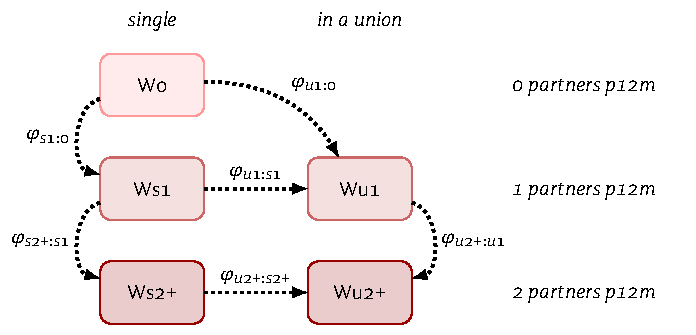
\includegraphics[scale=.8]{diag.nsw.adj}
  \caption{Illustration of how women (and equivalently men)
    are reallocated between union/partners in p12m strata
    based on odds ratios $\varphi$}
  \label{fig:model.nsw.adj}
  \floatfoot{\raggedright
    p12m: within the past 12 months
    W0: 0 partners in p12m;
    Ws1: single (not married/cohabiting) and 1 partner in p12m;
    Wu1: in a union (married/cohabiting) and 2+ partners in p12m;
    Ws2+: single and 2+ partners in p12m;
    Wu2+: in a union and 2+ partners in p12m.
    $\varphi$: odds of truly being in the second (arrowhead) vs first (tail) group.}
\end{figure}
%---------------------------------------------------------------------------------------------------
\paragraph{Union Status}
I assumed that under-reporting of main/spousal partnerships was minimal,
but that some ``main'' partnerships may not be captured in
the definition ``married/cohabiting'' from \cite{SDHS2006,SHIMS2};
thus $\varphi_{u1:0}$, $\varphi_{u1:s1}$, and $\varphi_{u2+:s2+}$
would be small but greater than 1
(horizontal transitions in Figure~\ref{fig:model.nsw.adj}).
Moreover, based on the median age of marriage, 23--29 \cite{SDHS2006},
approximately half of respondents aged 15--49 would have been married,
whereas only 28--39\% of women and men reported being in a union
(Figure~\ref{fig:Cwp.2006}~and~\ref{fig:Cwp.2016}),
although some marriages end in divorce/widowing \cite{SDHS2006}.
Thus, I sampled each of $\varphi_{u1:0}$, $\varphi_{u1:s1}$, and $\varphi_{u2+:s2+}$
from $1+\opname{Gamma}(\alpha,\beta=1)$
with $\alpha=.5$ for women and $\alpha=.3$ for men,
yielding mean (95\%~CI): 1.50~(1.00,~3.51) and 1.30~(1.00,~2.90), respectively.
%---------------------------------------------------------------------------------------------------
\paragraph{Partner Numbers}
Next, I defined $\varphi_{s1:0}$, $\varphi_{s2+:s1}$, and $\varphi_{u2+:u1}$ as follows
(vertial transitions in Figure~\ref{fig:model.nsw.adj}).
The median age of first sex in Eswatini was
approximately 18 for women and 19.5 for men \cite{SDHS2006}.
Thus, the 31--36\% of women and 34--41\% of men aged 15--49 reporting no partners in p12m
(Figure~\ref{fig:Cwp.2006}~and~\ref{fig:Cwp.2016}) is likely overestimated,
although some individuals may be abstinent in p12m following sexual debut.
I assumed that women had 3 and men had 2 times the odds of
actually having 1 casual partner in p12m while reporting no partners.
Thus, I sampled $\varphi_{s1:0}$ from $1+\opname{Gamma}(\alpha,\beta=1)$
with $\alpha=2$ for women and $\alpha=1$ for men,
yielding mean (95\%~CI): 3.00~(1.24,~6.57) and 2.00~(1.03,~4.69), respectively.
Drawing on \cite{Behanzin2013}, I assumed that ``single'' women and men (not married/cohabiting)
were less likely to report multiple partners in p12m, but women more so.
Thus, I sampled $\varphi_{s2+:s1}$ from $1+\opname{Gamma}(\alpha,\beta=1)$
with $\alpha=4$ for women and $\alpha=1$ for men,
yielding 5.00~(2.09,~9.77) and 2.00~(1.03,~4.69).
I made a similar assumption about married/cohabiting women and men,
with the same odds for men, but even greater odds of non-reporting among women.
I sampled $\varphi_{u2+:u1}$ from $1+\opname{Gamma}(\alpha,\beta=1)$
with $\alpha=6$ for women and $\alpha=1$ for men,
yielding 7.00~(3.20,~12.67) and 2.00~(1.03,~4.69).
%---------------------------------------------------------------------------------------------------
\subsubsection{Bias Adjustment: Resulting Group Sizes \& Partner Numbers}\label{model.par.nsw.res}
The mean resulting adjusted proportions $W'$ and $M'$
from solving the system with the assumed odds ratios $\varphi$
are illustrated in Figure~\ref{fig:Cwp.adj}, which can be compared to
the reported proportions in \sfref{fig:Cwp.2006}~and~\sfref{fig:Cwp.2016}.
Figure~\ref{fig:Cwp.adj.dens} also illustrates the empiric density distributions
for each element $W'_{i}$ and $M'_{i}$.
Numerically, the mean (95\%~CI) estimates were:
\begin{itemize}
  \item $W'_{0} = 17~(9,~27)$\% of women and $M'_{0} = 25~(13,~35)\%$ of men had 0 partners in p12m
  \item $W'_{1} = 66~(57,~75)$\% of women and $M'_{1} = 49~(37,~61)\%$ of men had 1 partners in p12m
  \item $W'_{2+} = 17~(10,~27)$\% of women and $M'_{2+} = 26~(15,~44)$\% of men had 2+ partners in p12m
  \item $W'_{u1} / W'_{01} = 38~(21,57)$\% women and $M'_{u1} / M'_{01} = 35~(23,~50)$\% men
    with 0--1 partners in p12m were in a main/spousal partnership
  \item $W'_{s1} / W'_{01} = 41~(19,65)$\% women and $M'_{s1} / M'_{01} = 31~(15,~55)$\% men
    with 0--1 partners in p12m were in a single casual partnership
  \item $W'_{u2+} / W'_{2+} = 32~(9,55)$\% women and $M'_{u2+} / M'_{2+} = 38~(13,~62)$\% men
    with 2+ partners in p12m were in a main/spousal partnership,
    and the rest had only casual partnerships.
\end{itemize}
%---------------------------------------------------------------------------------------------------
\paragraph{Group Sizes}
From these results, I defined the sizes of the modelled lower and medium activity groups,
and the average numbers of main/spousal partnerships per person.
I assumed that $W'_{2+}$ and $M'_{2+}$ included FSW and client population sizes, respectively
(see \sref{model.par.sw.size}).
Thus, the populations size of medium activity women was defined as
$P_{s_{1}i_{2}} = W'_{2+} - P_{s_{1}i_{34}}$.
Sampling $W'_{2+}$ from a BAB distribution with 95\%~CI (10,~27)\%,
the resulting 95\%~CI for medium activity women $P_{s_{1}i_{2}}$ was (6,~25)\% of women.
The lowest activity women population size was then defined as $1 - P_{s_{1}i_{234}}$,
representing (73,~90)\% of women.
Since there is greater uncertainty in the client population size,
the same approach for the medium activity men population size $P_{s_{2}i_{2}}$
could yield negative values.
Instead, I sampled $P_{s_{2}i_{2}}$ directly from
a BAB distribution with 95\%~CI (10,~17)\%, yielding
95\%~CI for $P_{s_{2}i_{234}}$ of (15,~50)\% of men,
which is close to (15,~44)\% from $M_{2+}$.
The lowest activity men were then then defined as $1 - P_{s_{2}i_{234}}$,
representing (50,~85)\% of men.
%---------------------------------------------------------------------------------------------------
\paragraph{Main/Spousal Partnerships}
To simplify model fitting, I sampled a common proportion of
individuals reporting a main/spousal partnership from a BAB distribution with 95\%~CI (25,~50)\%,
applied to all women and men in the lowest activity groups ($C_{p_{1}s_{12}i_{1}}$),
as well as all women in the median activity group ($C_{p_{1}s_{1}i_{2}}$).
Then, \eqrefs{eq:C2Q}{eq:C2K} were used to define $Q$ and $K$, respectively.
Since FSW and clients had fewer main/spousal partnerships (see \sref{model.par.nsw.sw}),
I calculated the proportion of men in the medium activity group having main/spousal partnerships
$K_{p_{1}s_{2}i_{2}}$ to balance the total number of main/spousal partnerships among women and men.
%---------------------------------------------------------------------------------------------------
\paragraph{Casual Partnerships}
I similarly defined a common proportion of women and men in the lowest activity groups
reporting casual partnership $C_{p_{2}s_{12}i_{1}}$ with 95\%~CI (20,~55)\%.
However, the number of casual partnerships among $W_{2+}$ and $M_{2+}$ ramains uncertain.
The analysis above provides no information on these values,
but the number of partners in p12m for the medium activity groups must be at least about 1.5
to ensure these women and men actually have 2+ partners in p12m.
Thus, I sampled the number of casual partners reported by women in the medium activity group
$C_{p_{2}s_{1}i_{2}}$ from a gamma distribution with 95\%~CI (1.2,~2),
and computed $Q$ and $K$ via \eqrefs{eq:C2Q}{eq:C2K}.
As before, I calculated the numbers of casual partnerships among men in the medium activity group
$K_{p_{2}s_{2}i_{2}}$ to balance total casual partnerships.
%---------------------------------------------------------------------------------------------------
\subsubsection{Main/Spousal \& Casual Partnerships among FSW \& Clients}\label{model.par.nsw.sw}
Among Swati FSW, the mean number of total non-paying partners in the past month was
approximately 1--1.5 (Table~\ref{tab:fsw.ratios}),
which may include both main/spousal partners and casual partners.
Among FSW in South Africa \cite{Wells2018} and Kenya \cite{Voeten2007},
while 54 and 72\% (respectively) reported being in a relationship, only 6 and 3\% were married,
although many non-marital partners may still constitute effectively ``main'' partnerships
with respect to condom use and duration.
Thus, I assumed that:
50\% of all FSW reported a main/spousal partner (\ie $C_{p_{1}s_{1}i_{34}} = 0.5$);
lower risk FSW reported $C_{p_{2}s_{1}i_{3}} = 0.5$ casual partners; and
higher risk FSW reported $C_{p_{2}s_{1}i_{4}} = 1.0$ casual partners, on average.
\par
Available data suggest that about half of clients also report non-sex work partners,
which are not always distinguished as main/spousal \vs casual partnerships
\cite{Lowndes2000,Santo2005}.
Non-paying partners of FSW are also often clients of other FSW \cite{Voeten2007,Godin2008}.
Yet, clients of FSW also tend to be younger and more likely to be
never/formerly married \vs non-client men \cite{Lowndes2000,Carael2006}.
So, I assumed that clients reported
half the numbers of main/spousal partnerships compared to lowest activity men:
$C_{p_{1}s_{2}i_{34}} = 0.5\,C_{p_{1}s_{2}i_{1}}$, and
25--100\% the numbers of casual partnerships compared to medium activity women (uniform prior).
As before, I computed $Q$ and $K$ via \eqrefs{eq:C2Q}{eq:C2K}.
%===================================================================================================
\subsection{Turnover}\label{model.par.turn}
%---------------------------------------------------------------------------------------------------
\subsubsection{Births \& Deaths}\label{model.par.turn.bd}
The modelled population considers ages 15--49,
reflecting commonly reported data and the majority of sexual activity.
In the absence of mortality, individuals would therefore
remain within the modelled ``open cohort'' population for 35 years.
The estimated average yearly mortality rate for these ages was 1.44\% around 2006
\cite[Table~15.2]{SDHS2006}.
However, this estimate includes HIV/AIDS-attributable mortality,
which I model separately (see \sref{model.par.hiv.mort}),
accounting for approximately 64\% of deaths around that time \cite{WHO2006esw}.
Thus, the overall exit rate from the modelled cohort
due to reaching age 50 (``aging out'') and non-HIV-attributable mortality was:
$\mu = 1/35 + (1-.64) 1.44\% = 3.78\%$.
\par
I estimated the rate of entry into the modelled population $\nu$
to fit population size of ages 15--49 in Eswatini \cite{WorldBank},
and approximate population growth rates \cite{UNWPP2019},
given that I model HIV/AIDS-attributable mortality separately.
Specifically, I assumed a population growth rate $g = \nu - \mu$ in the absence of HIV/AIDS of
4\% in 1980, 3\% in 2000, 1.5\% in 2010, and 1.5\% in 2020 (monotonic cubic interpolation).
I sampled $g$ in 2050 from a uniform prior with 95\% CI (0.7\%,~1.5\%),
reflecting uncertainty in estimated projections \cite{UNWPP2019}.
Finally, I calculated the population entry rate as $\nu = g + \mu$.
These parameter values were informally validated by comparison of model outputs with
Swati population sizes for ages 15--49 from \cite{WorldBank}.
The distribution of activity groups among individuals \emph{entering} the model, denoted $E_{si}$,
is different from the distribution among individuals \emph{currently} in the model $P_{si}$,
but $E_{si}$ is computed automatically as described below in \sref{model.par.turn.act}.
%---------------------------------------------------------------------------------------------------
\subsubsection{Activity Group Turnover}\label{model.par.turn.act}
In addition to overall population turnover (entry/exit from the open population),
I model movement of individuals between activity groups within the model.
Activity group turnover reflects the fact that risk is not constant over sexual life course,
and reported duration in higher activity contexts can be short \cite{Scorgie2012}.
Previous modelling has shown that activity group turnover (sometimes called ``episodic risk'')
can strongly influence parameter fitting and intervention impact \cite{Henry2015,Knight2020}.
I model turnover from activity group $si$ to $si'$ as a constant rate $\theta_{sii'}$,
which implies an assumption that (in the absence of HIV) duration in group $si$ is
exponentially distributed with mean $D_{si}$ \cite{Roberts2015}:
\begin{equation}\label{eq:model.par.dur}
  D_{si} = \frac{1}{\mu + \sum_{i'}\theta_{sii'}}
\end{equation}
where $\mu$ is the overall exit rate from \sref{model.par.turn.bd}.
As shown previously \cite{Knight2020}, the relative sizes of each sex-activity group $P_{si}$
can be maintained at fixed values by satisfying the following ``mass-balance'' equation:
\begin{equation}
  \nu P_{si} = \nu E_{si} + \sum_{i'} \theta_{si'i} P_{si'} - \sum_{i} \theta_{sii'} P_{si}
\end{equation}
Specific turnover rates $\theta_{sii'}$ and entrant activity group sizes $E_{si}$
can then be uniquely resolved by specifying
$N_i\,(N_i-1) = 12$ non-redundant and compatible constraints,
where specifying each $D_{si}$ is one such constraint.
%---------------------------------------------------------------------------------------------------
\paragraph{Duration Selling Sex}
The FSW survey data for 2011 \cite{Baral2014}, 2014 \cite{EswKP2014}, and 2021 \cite{EswIBBS2022}
include questions on the respondent's current age, and age of first selling sex;
the difference between these ages can then define a ``duration selling sex''.
Using this approach, the unadjusted years selling sex among Swati FSW were
median [IQR]: 4~[2,~7] in 2011 and 5~[3,~9] in 2014,
with histograms shown in Figure~\ref{fig:fsw.yss.raw}.
However, such estimates have three sources of bias:
sampling error, censoring, and measurement error.
\par
Sampling error was addressed through RDS-adjustment in 2011 and 2021,
yielding estimates of the proportions of FSW
who have been selling sex for 0--2, 3--5, 6--10, and 10+ years.
The adjusted proportions are not significantly different between 2011 and 2021, and
indicate fewer years selling sex \vs the unadjusted proportions, which would be consistent with
challenges in reaching women in the first year(s) of sex work \cite{Cheuk2020}.
I fit an exponential distribution to the cumulative adjusted proportions
(Figure~\ref{fig:fsw.yss.adj}), yielding an estimated distribution mean
${\lambda}^{-1}$ of 4.2~(3.5,~5.3) years.
However, the reported years selling sex in a cross sectional survey
will underestimate the eventual duration in sex work among respondents by a factor $f \le 2$,
because respondents continue selling sex after the survey
--- \ie the observed duration is right censored
(see \sref{app.model.math.xdur} for derivation and further discussion).
Thus, the overall mean duration in sex work would be given by $\bar{D} = f\,\lambda^{-1}$.
Yet, additionally, the current definition of duration selling sex
includes a hidden assumption that FSW sell sex continuously after starting.
In fact, 348/777 (45\%) FSW reported having ever stopped selling sex
in the 2014 survey \cite{EswKP2014} (other surveys did not ask).
Among these FSW, the expected duration selling sex in the current period
(\ie since re-starting most recently)
must be less than half ($\rho < 1/2$) of the durations calculated above.
Thus, an adjusted overall mean duration can be calculated as
$\bar{D} = (0.45\,\rho + 0.55)\,f\,\lambda^{-1}$.
Taking $\rho \sim \opname{Unif}(0.2,0.4)$ and $f \sim \opname{Unif}(1.5,2)$,
we obtain $\bar{D}$ with mean (95\%~CI): 5.13~(3.87,~6.72),
similar to the pooled estimate for African FSW up to 2010: 5.5~years~\cite{Fazito2012}.
\par
Finally, I assumed that higher risk FSW stay in sex work longer by a factor of
$R_{D}$ with 95\%~CI (1.54,~3.25) (gamma prior, Table~\ref{tab:fsw.ratios}).
Thus, durations in sex work among higher risk ($D_{HR}$) and lower risk ($D_{LR}$) FSW
can be resolved using:
\begin{equation}
  \begin{aligned}
    \bar{D} &= 0.2\,D_{HR} + 0.8\,D_{LR} \\
    R_{D} &= D_{HR} / D_{LR}
  \end{aligned}
\end{equation}
yielding mean (95\%~CI) $D_{LR}$: 4.07~(2.96,~5.48) and $D_{HR}$: 9.33~(6.30,~13.13) (gamma priors).
%---------------------------------------------------------------------------------------------------
\paragraph{Duration Buying Sex}
Data to inform the average duration spent buying sex among clients is limited.
\citet{Fazito2012} estimated mean durations of 4.6--5.5 years
based on studies in Benin \cite{Lowndes2000} and Kenya \cite{Voeten2002}.
\citet[Table~G]{Hodgins2022} also gives pooled estimates for
the proportions of men in Sub-Saharan Africa
who paid for sex \emph{ever} \vs in \emph{p12m} during 2000--2020.
Estimates ranged from 8.8~(6.5,~11.7)\% of men aged 25--34 who ever bought sex,
to 2.2~(1.5,~3.2)\% of men aged 35--54 who bought sex in p12m.
Based on these data, I defined a gamma prior distribution for the duration buying sex
with 95\%~CI (4,~15) years, applied to both higher and lower risk clients.
%---------------------------------------------------------------------------------------------------
\paragraph{Lowest \& Medium Activity Groups}
Data on individual-level changes to numbers of non-sex work partners in p12m
is even more sparse than data related to sex work;
so, it's unclear to what extent individuals move between the lowest and medium activity groups
throughout their sexual life course.
Data from Uganda, Zimbabwe, and South Africa \cite{Todd2009}
suggested that sexual activity (proportion sexually active and mean numbers of partners)
was approximately stable with age (after sexual debut and and before age 49),
with modest trends toward lower activity at older age.
However, these population-level data do not necessarily suggest that
the \emph{same} individuals have multiple partnerships each year.
Reflecting this uncertainty, I sampled
the rate of turnover from medium to lowest activity for both women and men
from a gamma prior with 95\%~CI (5,~50)\% per year.
%---------------------------------------------------------------------------------------------------
\paragraph{Additional Turnover Assumptions}
The above assumptions specify 3 key constraints for each sex:
two durations $D_{si}$ and one turnover rate $\theta_{sii'}$.
Since higher and lower risk FSW (and clients) are conceptualized as mutually exclusive groups,
I modelled no turnover between these groups:
$\theta_{si_{3}i'_{4}} = \theta_{si_{4}i'_{3}} = 0$ (+2~constraints).
Next, since FSW often enter sex work shortly after sexual debut \cite{Cheuk2020,Ma2020},
and sexual activity is roughly constant or slightly declining with age \cite{Todd2009},
I assumed that $E_{si} = f\,P_{si}$,%
\footnote{Subject to $f \le (\nu - \mu + D_{si}^{-1})\,\nu^{-1}$,
  which can be derived from Eq.~(10) in \cite{Knight2020}.}
with $f = 2$ for FSW, $f = 1.5$ for clients,
and $f = 1$ for medium activity women and men (+3~constraints);
then $f < 1$ for the lowest activity women and men is computed automatically.
Finally, since exiting sex work is unlikely to be
an abrupt transition to monogamous or zero sexual activity \cite{Scorgie2012,Learmonth2015},
I further assumed that (50,~90)\% of women exiting sex work
transition to the medium activity group (BAB prior) (+1~constraint);
in the absence of relevant data, I made a similar assumption regarding clients,
with (25,~90)\% former clients transitioning to the medium activity group (+1~constraint).
These $10 < 12$ total constraints then allow two degrees of freedom to resolve
the values of $\theta_{sii'}$ and $E_{si}$.
A non-negative solution to the system of constraints is solved as described in \cite{Knight2020},%
\footnote{Using \hreftt{docs.scipy.org/doc/scipy/reference/generated/scipy.optimize.nnls.html}}
repeated at each timestep as $\nu$ varies with time.
%===================================================================================================
\subsection{Sex Frequency \& Partnership Duration}\label{model.par.sex}
%---------------------------------------------------------------------------------------------------
\subsubsection{Sex Frequency}\label{model.par.sex.freq}
The Eswatini general population data sources \cite{SDHS2006,SHIMS1,SHIMS2}
did not report on frequency of sex. % yes they did, SDHS2006: Table 6.10 TODO
In South Africa, average numbers of sex acts per week per partnership (non-sex work)
was reported as mean 2.5~(IQR: 1--3) \cite{Delva2013},
with consistent reports across main/spousal partnerships and casual partnerships.
Sex frequency among South Africans per month overall (not per-partnership)
is also summarized in \cite[Figure~3.15]{Shisana2005},
which is roughly consistent with \cite{Delva2013}, but motivates a smaller lower bound.
Median sex frequency per partnership-year in 1998 Rakai, Uganda was
approximately 90 acts with the ``more frequent'' of concurrent partners, and
approximately 20 acts with the ``less frequent'' \cite{Morris2010}.
Considering these data,
I sampled the number of sex acts per year in main/spousal partnerships
$F_{p_{1}}$ from a gamma prior distribution with 95\%~CI (13,~156),
and a relative rate for casual partnerships $F_{p_{2}}/F_{p_{1}} \sim \opname{Unif}(0.5,1)$.
As described in \sref{model.par.sw.part},
I defined $F_{p_{3}} = 12$ for occasional sex work partnerships,
and $F_{p_{4}} \sim \opname{Unif}(12,36)$ for regular sex work partnerships.
I also constrained samples of $F_{p_{4}}$ such that
higher risk FSW never have commercial sex more than twice daily, on average.
% Coital frequency is not thought to be influenced by concurrent partnerships \cite{Delva2013}.
%---------------------------------------------------------------------------------------------------
\subsubsection{Anal Sex}\label{model.par.sex.anal}
Among Eswatini data sources, only \cite{EswKP2014} (FSW, 2014)
counted sex acts separately for anal and vaginal sex.
Among all FSW, the proportion of ``average sex acts per week'' that were anal (vs vaginal) was 2.9\%.
However, a previous coital diary study in neighbouring KwaZulu-Natal suggested
much higher proportions were anal \cite{Ramjee1999},
and face-to-face interview survey design may result in under-reporting \cite{Owen2020}.
Owen et al. review studies of anal sex in South Africa, and estimate that
0.6--16.5\% of sex acts among the general population are anal \cite{Owen2017}, \vs
2.4--15.9\% among FSW \cite{Owen2020}.
To reflect this greater uncertainty, the proportions of sex acts which are anal
in all partnerships were sampled from a gamma prior distribution with 95\%~CI (0.6,~16.5)\%.
%---------------------------------------------------------------------------------------------------
\subsubsection{Partnership Duration}\label{model.par.sex.dur}
As explored in Chapter~\ref{foi}, the durations of sexual partnerships
can be key determinants of epidemic dynamics and intervention impact.%
\footnote{Chapter~\ref{foi} also discusses the related phenomenon of partnership concurrency,
  including how concurrency is represented in compartmental models.}
Eswatini-specific data on partnership duration are lacking.
Moreover, accurate estimation of partnership duration remains challenging even when data exist,
due to censoring, truncation, and sampling biases \cite{Burington2010}.
Similar to challenges in estimating sex work duration (\sref{app.model.math.xdur}),
we must distinguish the definition of an ``average partnership'' as
(a) among all partnerships in a population over a given \emph{time period}, \vs
(b) among all partnerships in a population \emph{cross-section}.
Case (b) will be biased by partnership duration,
so the estimated mean duration will longer,
while case (a) reflects an unbiased estimate.%
\footnote{If case (a) durations are exponentially distributed,
  the durations in case (b) will be gamma-distributed with $\alpha = 2, \beta = \lambda$;
  thus the mean duration in case (b) will be $\alpha/\beta = 2\lambda$ (twice as long).}
The difference between the exponential distribution mean and median
should also be kept in mind (see \sref{app.model.math.exp}).
%---------------------------------------------------------------------------------------------------
\paragraph{Main/Spousal Partnerships}
Detailed data on marriage in Eswatini was only captured in 2006 \cite[Table~6.1]{SDHS2006}.
The median age of first marriage was 24.3 among women and 27.7 among men (26.0 overall).
Approximately 64\% of women and 88\% of men (76\% overall) who were ever married or living together
were in a union at age 50--54.
However, no data indicated whether any respondents had remarried or entered into a secondary union.
Among women aged 40--49, the most recent data on
median age of first marriage and proportions ever remarried were
33 years old and 6.6\% in South Africa,
20.9 and 3.7\% in Lesotho, and 18.7 and 28.4\% in Mozambique \cite{John2022};
such data may not capture non-marital secondary unions.
Thus, I assumed $\rho = {}$5--20\% of unions among EmaSwati aged 50--54 were secondary.
Considering that the modelled population only includes ages 15--49,
I then defined the mean durations of main/spousal partnerships as
$\delta_{p_{1}} =  (0.76 - \rho)\,(49 - 26) \in (14.5, 18.5)$ years.
\par
In some models, partnership duration is used to define both
the total numbers of sex acts per partnership and the partnership change rate (see \sref{foi.prior}).
This change rate might be overestimated by the above definition,
since the rate should also consider whether and when
divorced/separated individuals form \emph{new} main/spousal partnerships.
The change rate could even be tied to the modelled baseline and HIV-attributable mortality,
given that the majority of Swati unions ended via spousal death
(83\% of unions among women and 56\% among men by age 50--54) \cite{SDHS2006}.
% TODO: (?) add exit from "k=1" state, rate proportional to HIV-attrib-mort of opposite sex
For simplicity and consistency with prior approaches,
I used the effective duration of 14.5--18.5 years throughout (uniform prior).
%---------------------------------------------------------------------------------------------------
\paragraph{Casual Partnerships}
No data is available regarding durations of non-marital sexual partnerships in Eswatini,
and regional data on are also limited.
I synthesized the available partnership duration data from
South Africa \cite{Harrison2008,Hargreaves2009,Nguyen2015},
Rural Tanzania \cite{Nnko2004},
and four cities in Kenya, Zambia, Benin, and Cameroon \cite{Ferry2001}.
Based on these data, I defined a gamma prior distribution for
the mean duration of casual partnerships $\delta_{p_{2}}$ with 95\%~CI (0.25,~1.5) years,
roughly consistent with prior models \cite{Johnson2009}.
%---------------------------------------------------------------------------------------------------
\paragraph{Sex Work Partnerships}
As noted in \sref{model.par.sw.part}, duration of occasional sex work partnerships
is ill defined, but can be defined to comprise a single sex act with $F_{p_{3}}\delta_{p_{3}} = 1$.
Data on regular sex work partnerships is severely limited, and
sometimes regular paying clients later become
non-paying emotional partners \cite{Voeten2007,Mbonye2022}.
Based on \cite{Voeten2002}, I defined a gamma prior distribution for
the mean duration of regular sex work partnerships $\delta_{p_{4}}$ with 95\%~CI (0.5,~2.0) years.
% TODO: is this too long given FSW turnover?
%===================================================================================================
\subsection{Mixing}\label{model.par.mix}
In addition to more concentrated transmission
among FSW and their clients via regular and occasional sex work partnerships
--- which are \emph{only} formed among FSW and clients ---
other types of partnerships may be formed
preferentially between particular activity groups.
For example, FSW and clients may be more likely to form main or casual partnerships
with each other than with other activity groups.
Such preferences are captured in a ``mixing matrix'' $M$, where $M_{pii'}$ denotes
the total number of type-$p$ partnerships formed between groups $i$ and $i'$ in the population
(ignoring sex indices $s,s'$ temporarily)
--- \ie who has sex with whom.
The mixing matrix $M_{pii'}$ must be symmetric,
and have row/column sums equal to the total numbers of partnerships ``offered'' by any group:
$M_{pi} = P_{i} C_{pi}$ (group size $\times$ partnerships per-person).
%---------------------------------------------------------------------------------------------------
\subsubsection{Classic $\epsilon$ Mixing}\label{model.par.mix.eps}
In many risk/activity-stratified compartmental transmission models,
mixing is parameterized via a single parameter $\epsilon \in [0,1]$,
which controls the degree of like-with-like mixing \cite{Nold1980}.
This approach is often attributed to \cite{Garnett1994},
wherein a key adjustment for imbalanced partner numbers among women \vs men was introduced.
The approach defines the \emph{probability} of
someone from group $i$ forming a \emph{given} type-$p$ partnership with someone from group $i'$ as:
\begin{equation}\label{eq:mix.eps}
  \rho_{pii'} = (\epsilon)\,I_{ii'} + (1 - \epsilon)\,\pi_{ii'},
  \quad I_{ii'} = \begin{cases} ~1 & i = i'\\ ~0 & i \ne i' \end{cases},
  \quad \pi_{ii'} = \frac{M_{pi'}}{\sum_{j}M_{pj}}
\end{equation} where:
$I$ represents complete like-with-like mixing (an identity matrix),
$\pi$ represents random mixing (random but proportional to the number of partnerships ``offered''),
and $\epsilon$ effectively interpolates between these two extremes.
Thus, $\epsilon = 0$ reflects fully random mixing,
and $\epsilon = 1$ reflects fully like-with-like mixing.
Then, the total numbers of type-$p$ partnerships between groups $i$ and $i'$ can be
defined as $M_{pii'} = M_{pi}\,\rho_{pii'}$.
Three advantages of \eqref{eq:mix.eps} are:
(1) simplicity;
(2) $\epsilon$ can be directly interpreted as the proportion of partnerships
which are formed among like-with-like \vs randomly; and
(3) it guarantees that $M$ will be symmetric, even if $P$ and/or $C$ change.
Yet, the simplicity of this approach precludes implementation of more complex mixing patterns,
although some modest extensions can be made,
such as asymetric age mixing among women and men (\eg \cite{Cremin2013}).
%---------------------------------------------------------------------------------------------------
\subsubsection{Log-Linear Mixing}\label{model.par.mix.ll}
A more general  approach to mixing is developed in \cite{Morris1991}.
This ``log-linear'' approach defines the mixing matrix elements $M_{pii'}$ as follows.
The expected total numbers of partnerships between risk groups under random mixing are defined as:
\begin{equation}\label{eq:mix.rand}
  \Pi_{pii'} = \frac{M_{pi} M_{pi'}}{\sum_{j} M_{pj}}
\end{equation}
% TODO: add later $\theta$ / $\omega \in [0,1]$ if # offered partners don't balance
Next, a matrix $\Phi_{pii'}$ is defined, representing the odds of
a type-$p$ partnership forming between groups $i$ and $i'$, compared to random mixing.
The matrix $\Phi$ must be symmetric,
and can be estimated directly from the right kind of data
(which is rarely available) \cite{Morris1991}.
Then, an initial estimate of $M_{pii'}$ is:
\begin{alignat}{1}
  M_{pii'}^{\,(0)} &= \exp{\left[\log{\left(\Pi_{pii'}\right)} + \Phi_{pii'} \right]} \nonumber\\
                 &= \Pi_{pii'} \exp{\left(\Phi_{pii'}\right)} \label{eq:mix.M0}
\end{alignat}
However, this estimate changes the total numbers of partnerships formed by each group:
$M_{pi}^{\,(0)} \ne \Pi_{pi}$, where
$M_{pi} = \sum_{i'} M_{pii'}$ and $\Pi_{pi} = \sum_{i'} \Pi_{pii'}$.
There is no \textit{a priori} definition of $M_{pii'}$ or adjustment to $\Phi_{pii'}$
that can guarantee the numbers of partnerships will not change.%
\footnote{I hypothesize that this lack of \textit{a priori} solution
  is the reason this approach has not been widely used.}
However, an iterative proportional fitting procedure \cite{Ruschendorf1995}
can resolve an estimate $M_{pii'}^{\,(n)}$ that maintains the total numbers of partnerships:
\begin{equation}\label{eq:mix.iter}
  M_{pii'}^{\,(n+1)} = M_{pii'}^{\,(n)} \frac{\Pi_{pf}}{M_{pf}^{\,(n)}}
  \qquad f = \begin{cases}
    ~i  & \txn{if $n$ is even} \\
    ~i' & \txn{if $n$ is odd}
  \end{cases}
\end{equation}
Each step of this procedure can be understood as
a re-scaling of the current estimate $M_{pii'}^{\,(n)}$
row-wise ($i$) or column-wise ($i'$) to match the numbers of partnerships
offered by individuals ($\Pi_{pi}$) or their partners ($\Pi_{pi'}$).
Each row-step re-introduces discrepancies in the columns, and vice versa,
but overall convergence is guaranteed \cite{Sinkhorn1964}.
\par
In practice, \eqref{eq:mix.iter} adds approximately
one decimal of precision per $2n$ for the $4\times4$ case,
thus 15--20 iterations is often sufficient to come within computational precision limits.
Since the partnerships matrix $M_{pii'}$ should adapt to reflect changes in
group sizes (\eg due to HIV mortality) or
numbers of partnerships offered (\eg see \sref{foi.prop}),
the matrix must be re-computed at every time point.
Thus, the procedure \eqref{eq:mix.iter} could be considered computationally expensive.
However, this approach provides great flexibility and interpretability
to specify complex mixing patterns via the odds matrix $\Phi_{pii'}$.
\par
Adding back the sex dimension indices $i \rightarrow si, ~ i' \rightarrow s'i'$,
two final adjustments are needed for the bipartite (\ie heterosexual) system.
First, I ensure that $M_{s=s'} = \Pi_{s=s'} = 0$.
Second, for the case when the total numbers of partnerships offered by women and men
do not balance ($\sum_j M_{ps_{1}j} \ne \sum_j M_{ps_{2}j}$),
I revise the denominator of \eqref{eq:mix.rand} to $\sum_{j} \omega_s M_{psj}$,
where $\omega_s$ are weights such that $\sum_s \omega_s = 1$.
Similar to the ``compromise'' parameter $\theta$ in \cite{Garnett1994},
if $\omega = \{1,0\}$, then women's partnership numbers are matched exactly
while men adapt their partner numbers to balance;
and conversely for $\omega = \{0,1\}$.
I fixed $\omega = \{0.5,0.5\}$ for equal adaptation among women and men.
%---------------------------------------------------------------------------------------------------
\subsubsection{Odds of Mixing}\label{model.par.mix.odds}
Despite the flexibility in the odds of mixing matrix $\Phi_{pii'}$,
limited data are available to inform specific elements,
especially for Eswatini in particular.
In Kenya \cite{Voeten2007}, Benin, Guinea, and Senegal \cite{Godin2008}, and Uganda \cite{Mbonye2022},
a disproportionate fraction of non-paying partners of FSW were former and/or current clients.
Given this fraction $\psi$ and the proportion of all men who are clients $\rho$,
the odds of these partnerships forming can be computed as:
\begin{equation}
  \Phi = \frac{\psi\,(1-\rho)}{(1-\psi)\,\rho}
\end{equation}
Taking $\psi \in (0.33,~0.70)$ \cite{Voeten2007,Godin2008}
and $\rho \in (5,~20)\%$ \cite{Hodgins2022}, we obtain $\Phi \in (2,~19)$.
As noted in \sref{model.par.nsw.sw}, its not clear whether such partnerships reflect
main/spousal or casual partnerships.
As such, I sampled a common value for both partnership types,
as well as for higher/lower risk FSW and clients:
$\Phi_{p_{12}i_{34}i'_{34}}$ from a gamma prior with 95\%~CI of (2,~19).
I further assumed that lowest activity women and men had
greater odds of forming main/spousal partnerships with each other,
based loosely on age cohorting effects \cite{Leclerc-Madlala2008},
observed like-with-like sexual mixing preferences in numerous other contexts
\cite{Morris1991,Garnett1993a,Admiraal2016},
and prior modelling work \cite{Knight2022sr}.
I sampled $\Phi_{p_{1}i_{1}i'_{1}}$ from a gamma prior with 95\%~CI of (1.5,~3).
I made no further assumptions about preferential mixing (\ie all other elements $\Phi = 1$).
Thus, I assumed that occasional and regular sex work partnerships form
randomly with respect to higher \vs lower FSW and their clients.
